\documentclass[mathserif,10pt]{beamer}
% insert "handout" into the options argument of the documentclass
\usetheme{CambridgeUS}
\usecolortheme{beaver}
\usepackage{amsmath}
\usepackage{graphicx}
\usepackage{epstopdf}
\usepackage{xcolor}
%\usepackage{epstopdf}
%\usepackage{pdfpages}
\usepackage{media9}
%\usepackage{mdframed}
\DeclareGraphicsRule{.tif}{png}{.png}{`convert #1 `dirname #1`/`basename #1 .tif`.png}
\usepackage{hyperref}
%\usepackage[T1]{fontenc}
\usepackage{cancel}
\usepackage{tcolorbox}

\setbeamertemplate{navigation symbols}{}
\setbeamertemplate{items}[triangle]
\setbeamertemplate{section in toc}[ball unnumbered]

% Create a custom colour for alert boxes
\definecolor{myred}{RGB}{144,0,2}
\newtcolorbox{mybox}[1][]{
colback=myred,
colframe=myred,
colupper=white
}

%\setbeamercolor{button}{bg={\usebeamercolor[fg]{alerted text} red}, fg=white}

%\addtobeamertemplate{footline}{\insertframenumber / \inserttotalframenumber}

% To show TOC with current section highlighted at the 
% beginning of each section
\AtBeginSection[]
{
  \begin{frame}
  \frametitle{}
  \tableofcontents[currentsection]
  \end{frame}
}

% To turn off section review slide for a section
% { 
%  \AtBeginSection[]{}
%    \section{Example}
%    \frame{Example}
% }


\title[Gravitational Collapse in AdS]{Gravitational Collapse in Anti-de Sitter Space}
\author[Brad Cownden]{Brad Cownden \\ PhD Thesis Defence}
\date[July 28th, 2020]{July 28th, 2020}


\newcommand{\bi}{\begin{itemize}}
\newcommand{\ei}{\end{itemize}}
\newcommand{\its}{\item}
\newcommand{\be}{\begin{align*}}
\newcommand{\ee}{\end{align*}}
\newcommand{\td}{\tilde}
\newcommand{\wtn}{\widetilde{\nabla}}
\newcommand{\del}{\nabla}
\newcommand{\h}{\hat}
\newcommand{\p}{\partial}
\newcommand{\til}{\tilde}
\newcommand{\w}{\wedge}
\newcommand{\sh}{\hat\star}
\newcommand{\st}{\tilde\star}
\newcommand{\mc}{\mathcal}
\newcommand{\sla}{\slashed}
\newcommand{\scr}{\scriptsize}
\newcommand{\jm}{j_{max}}

\begin{document}

%%%%%%%%%%%%%%%%%%%%%%%%%%%%%%%%%%%%%%%%%%%%%%
%%%%%%%%%%%%%%%%%%%%%%%%%%%%%%%%%%%%%%%%%%%%%%

\frame
{
   \titlepage
   \begin{center}
   
\includegraphics[scale=0.25]{newlogos}
   \end{center}
}

\frame
{
  \frametitle{Outline}
  \tableofcontents
}

%%%%%%%%%%%%%%%%%%%%%%%%%%%%%%%%%%%%%%%%%%%%%%
%%%%%%%%%%%%%%%%%%%%%%%%%%%%%%%%%%%%%%%%%%%%%%
{
  \AtBeginSection[]{}
\section{Gravitational Collapse}
\frame
{
  \frametitle{Gravitational Collapse}
  \bi
  \its AdS/CFT\footnote<1->{{\scr Maldacena [hep-th/9711200]}} $\to$ thermal quench in gauge theory $\Leftrightarrow$ formation of black hole in gravitational theory
  \its Massless scalar fields in AdS: unstable against generic initial data, no minimum amplitude\footnote<1->{{\scr Bizo\'n \& Rostworowski [1104.3702]}} $\to$ c.f. Minkowski\footnote<1->{{\scr Choptuik PRL70 9 (1993)}} 
  \its Stability for specific initial data below critical amplitude
  \its {\bf Nonlinear theory:} continue\footnote<1->{{\scr Deppe \& Frey [1508.02709]}} with exploration of phase space
  \its {\bf Perturbative theory:} effects of truncation, space of solutions, time-dependent boundary conditions
  \ei	
}

%%%%%%%%%%%%%%%%%%%%%%%%%%%%%%%%%%%%%%%%%%%%%%
%%%%%%%%%%%%%%%%%%%%%%%%%%%%%%%%%%%%%%%%%%%%%%

\section{Massive Scalars in AdS$_5$}
\frame[c, noframenumbering]
{
  \frametitle{}
  \begin{center}
    \begin{mybox}[]
    B Cownden, N Deppe, and AR Frey, {\it Phase Diagram of Stability for Massive Scalars in Anti-de Sitter Spacetime}, Phys.Rev.D 102 (2020) 026015, [1711.00454].
    \end{mybox}
  \end{center}
}

%%%%%%%%%%%%%%%%%%%%%%%%%%%%%%%%%%%%%%%%%%%%%%

\subsection{Scalar Field Collapse in AdS}
\frame
{
  \frametitle{Scalar Field Collapse in AdS}
  \vspace{-0.7in}
  \bi
  \its Minimally-coupled scalar field in AdS$_5$ (dual to 4D CFT)
  \its Spherical symmetry, Schwarzschild-like coordinates $\to$ \alert<1>{$A(t,x)$}, \alert<1>{$\delta(t,x)$}
  \its Horizon formation when $A(t_H, x_H) \ll 1$
  \uncover<2->{\its Einstein equations $\Rightarrow$ constraints}
  \uncover<2->{\its Klein-Gordon equations $\Rightarrow$ dynamics}
  \uncover<2->{\its Examine behaviour near critical amplitude for different \alert{masses}, \alert{widths}}
  \ei

  \vspace{-0.2in}
  \begin{overlayarea}{\textwidth}{0.1cm}
    \begin{align*}
    \only<1>{
     ds^2 &= \frac{\ell^2}{\cos^2 (x/\ell)} \left( - \alert<1>{Ae^{-2\delta}} dt^2 + \alert<1>{A^{-1}} dx^2 + \sin^2 (x/\ell) d\Omega^{d-1} \right)
     }
     \only<2>{
     		\p_x M_{\text{ADM}} &= \frac{\tan^{d-1}(x)}{2} \left( A (\Pi^2 + \Phi^2) + \frac{\alert{\mu^2} \phi^2}{\cos^2(x)} \right) \\
    		\Pi(t=0, x) &= \epsilon \exp \left( - \frac{\tan^2(x)}{\alert{\sigma^2}} \right) \qquad \text{Phase space:} \: (\alert{\mu, \; \sigma})
    }
    \end{align*}
  \end{overlayarea}
  \vfill
}

%%%%%%%%%%%%%%%%%%%%%%%%%%%%%%%%%%%%%%%%%%%%%%

\subsection{Classifying Phases}

\frame
{
  \frametitle{Stable vs Unstable Profiles}
  \begin{center}
  Blue dot $=$ collapse detected, red triangle $=$ no collapse detected for $t \leq t_{max}$
  \end{center}
  \vspace{-0.1in}
  \begin{columns}
    \column{0.4\textwidth}
    \vspace{-0.25in}
    \bi
    \its Stable: abrupt jump in $t_H$ when $\epsilon < \epsilon_{crit}$
    \its<2->{Unstable: fit $t_H \approx a \epsilon^{-p} + b$ for $t_H \geq 60$ $\to$ perturbatively unstable when $p \approx 2$ (TTF)}
    \ei
    \column{0.6\textwidth}
    \begin{figure}
      \centering
      \only<1>{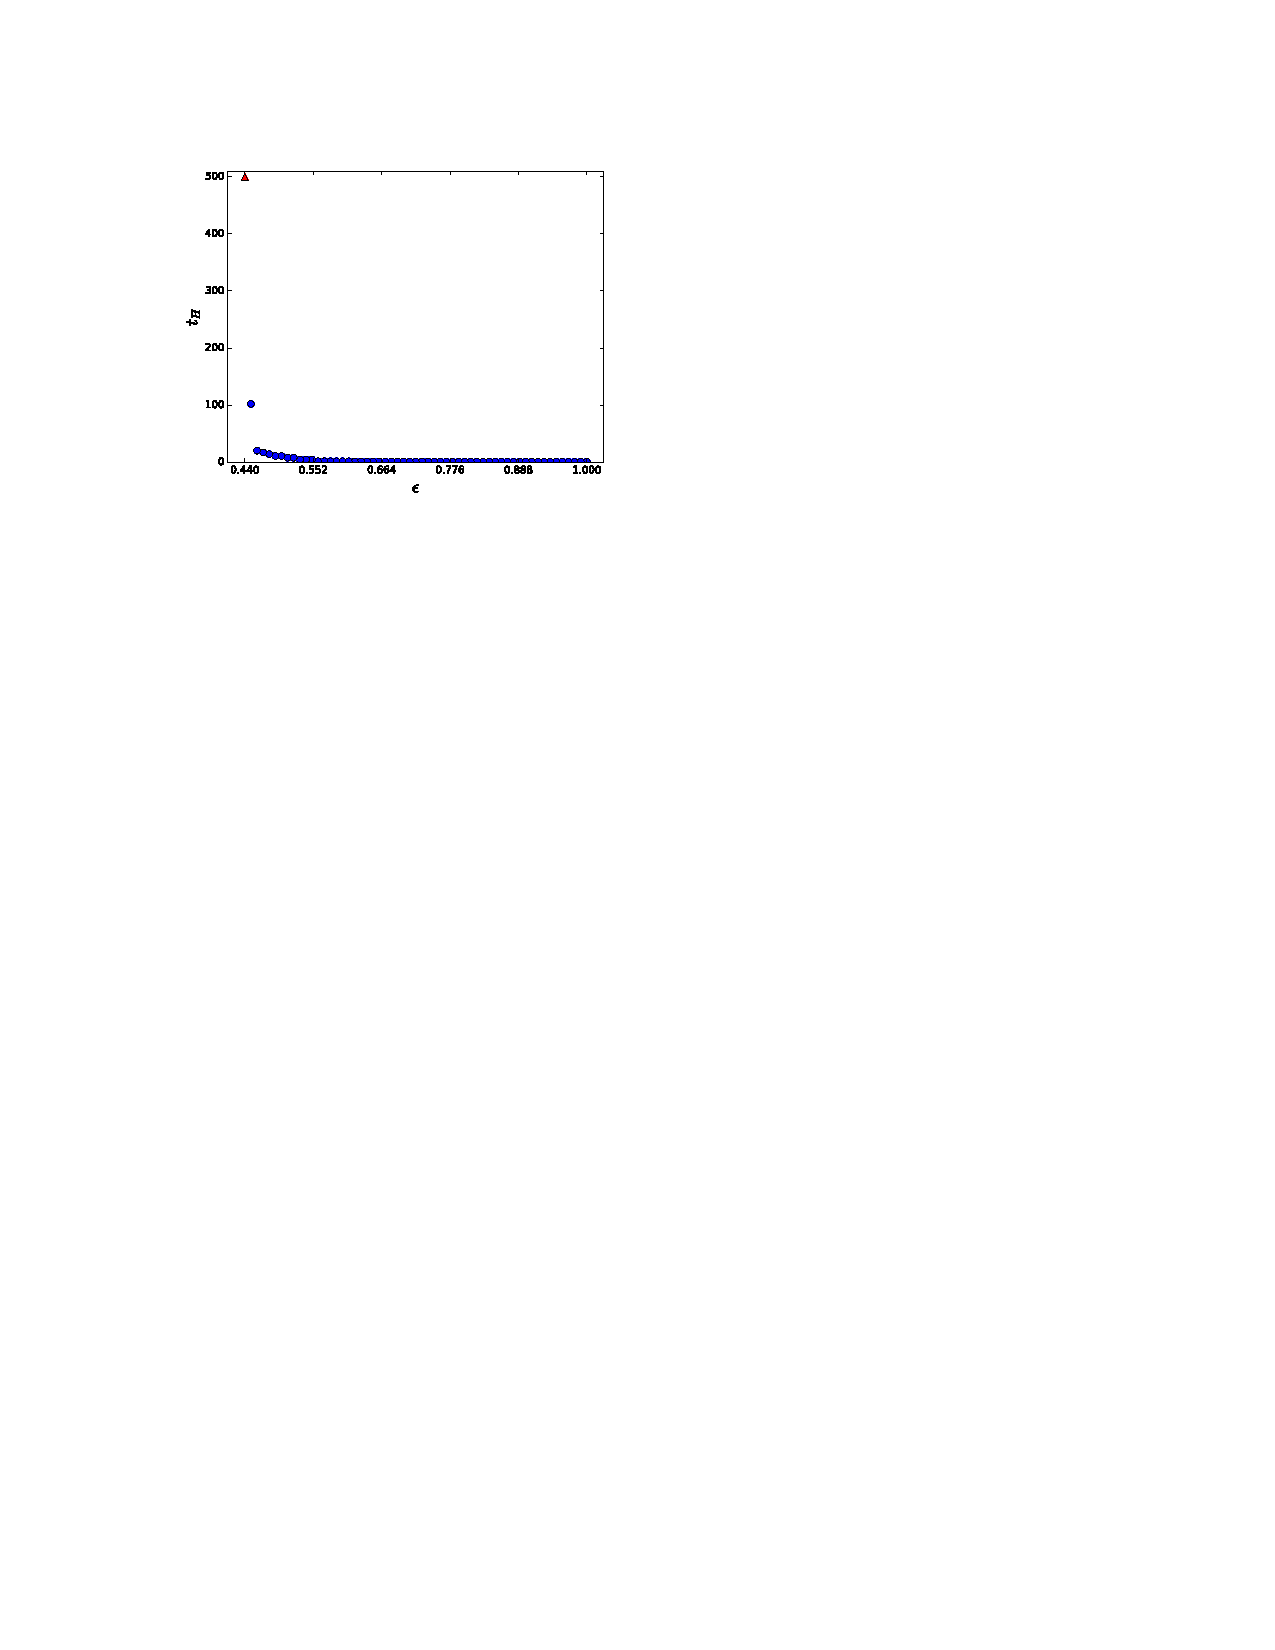
\includegraphics[width=\textwidth]{m0w15} \\ $\mu =0$, $\sigma =1.5$}
      \only<2>{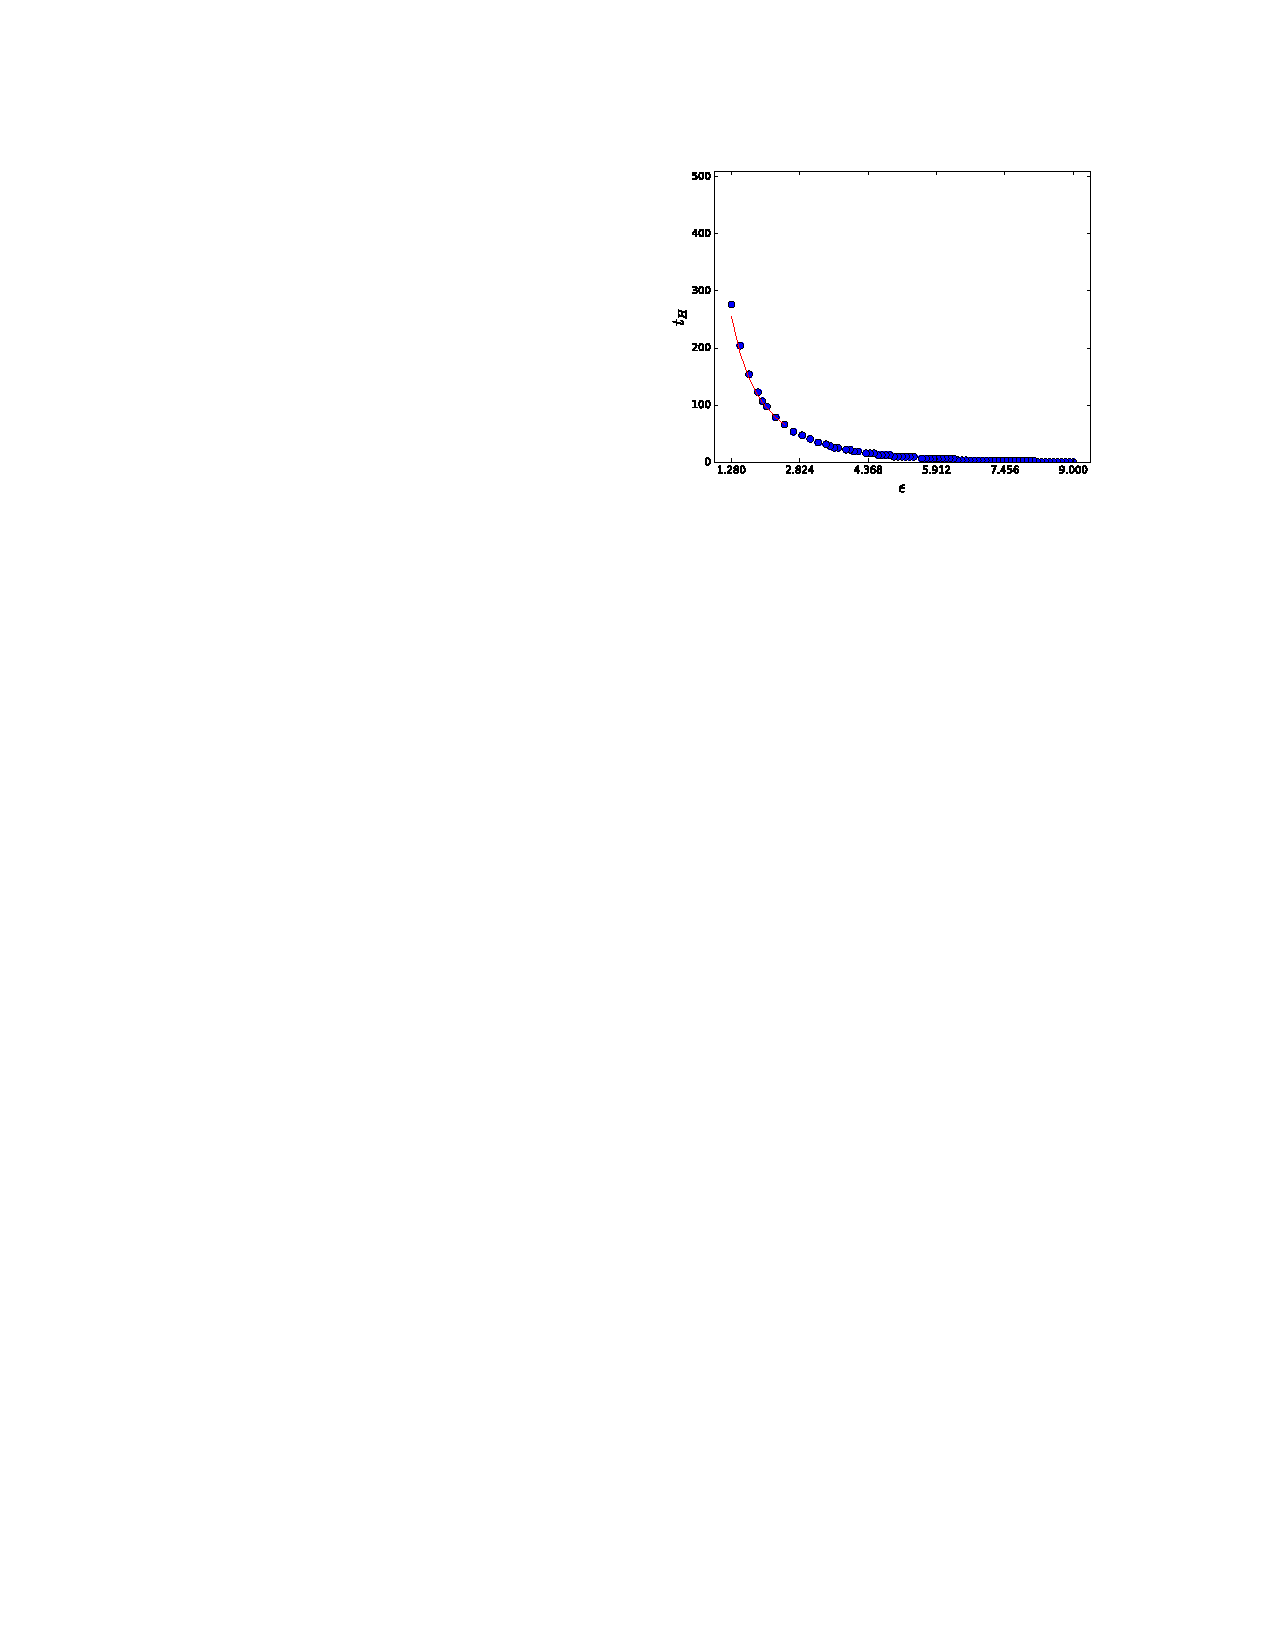
\includegraphics[width=\textwidth]{m0w025} \\ $\mu = 5$, $\sigma=0.25$}
    \end{figure}
 \end{columns}
}

\frame
{
  \frametitle{Metastable \& Irregular Profiles}
  \begin{center}
  Blue dot $=$ collapse detected, red triangle $=$ no collapse detected for $t \leq t_{max}$
  \end{center}
  \vspace{-0.1in}
  \begin{columns}
    \column{0.4\textwidth}
    \vspace{-0.25in}
    \bi
    \its Metastable: fit $t_H \approx a \epsilon^{-p} + b$ for $t_H \geq 60$ $\to$ $p > 2$
    \its<2->{Irregular: no scaling}
    \ei
    \column{0.6\textwidth}
    \begin{figure}
      \centering
      \only<1>{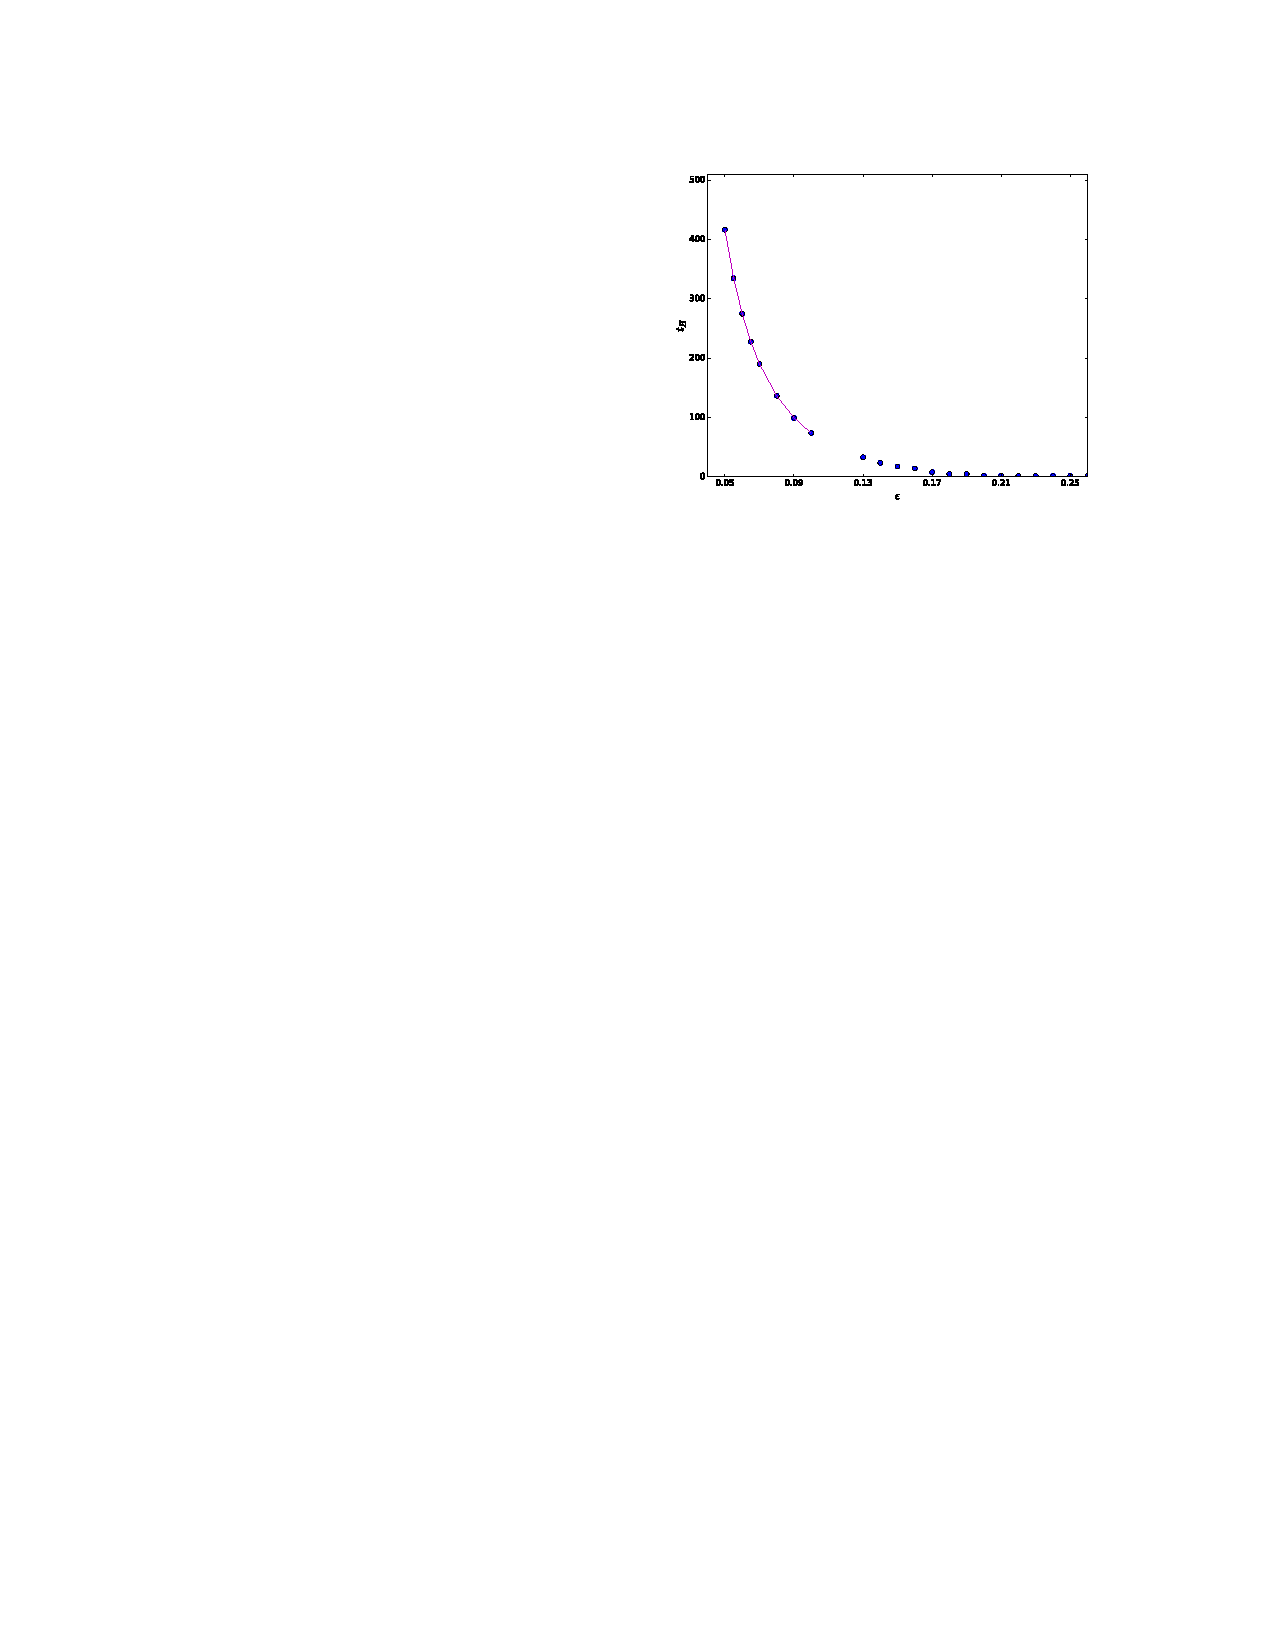
\includegraphics[width=\textwidth]{m5w17} \\ $\mu = 5$, $\sigma = 1.7$}
      \only<2>{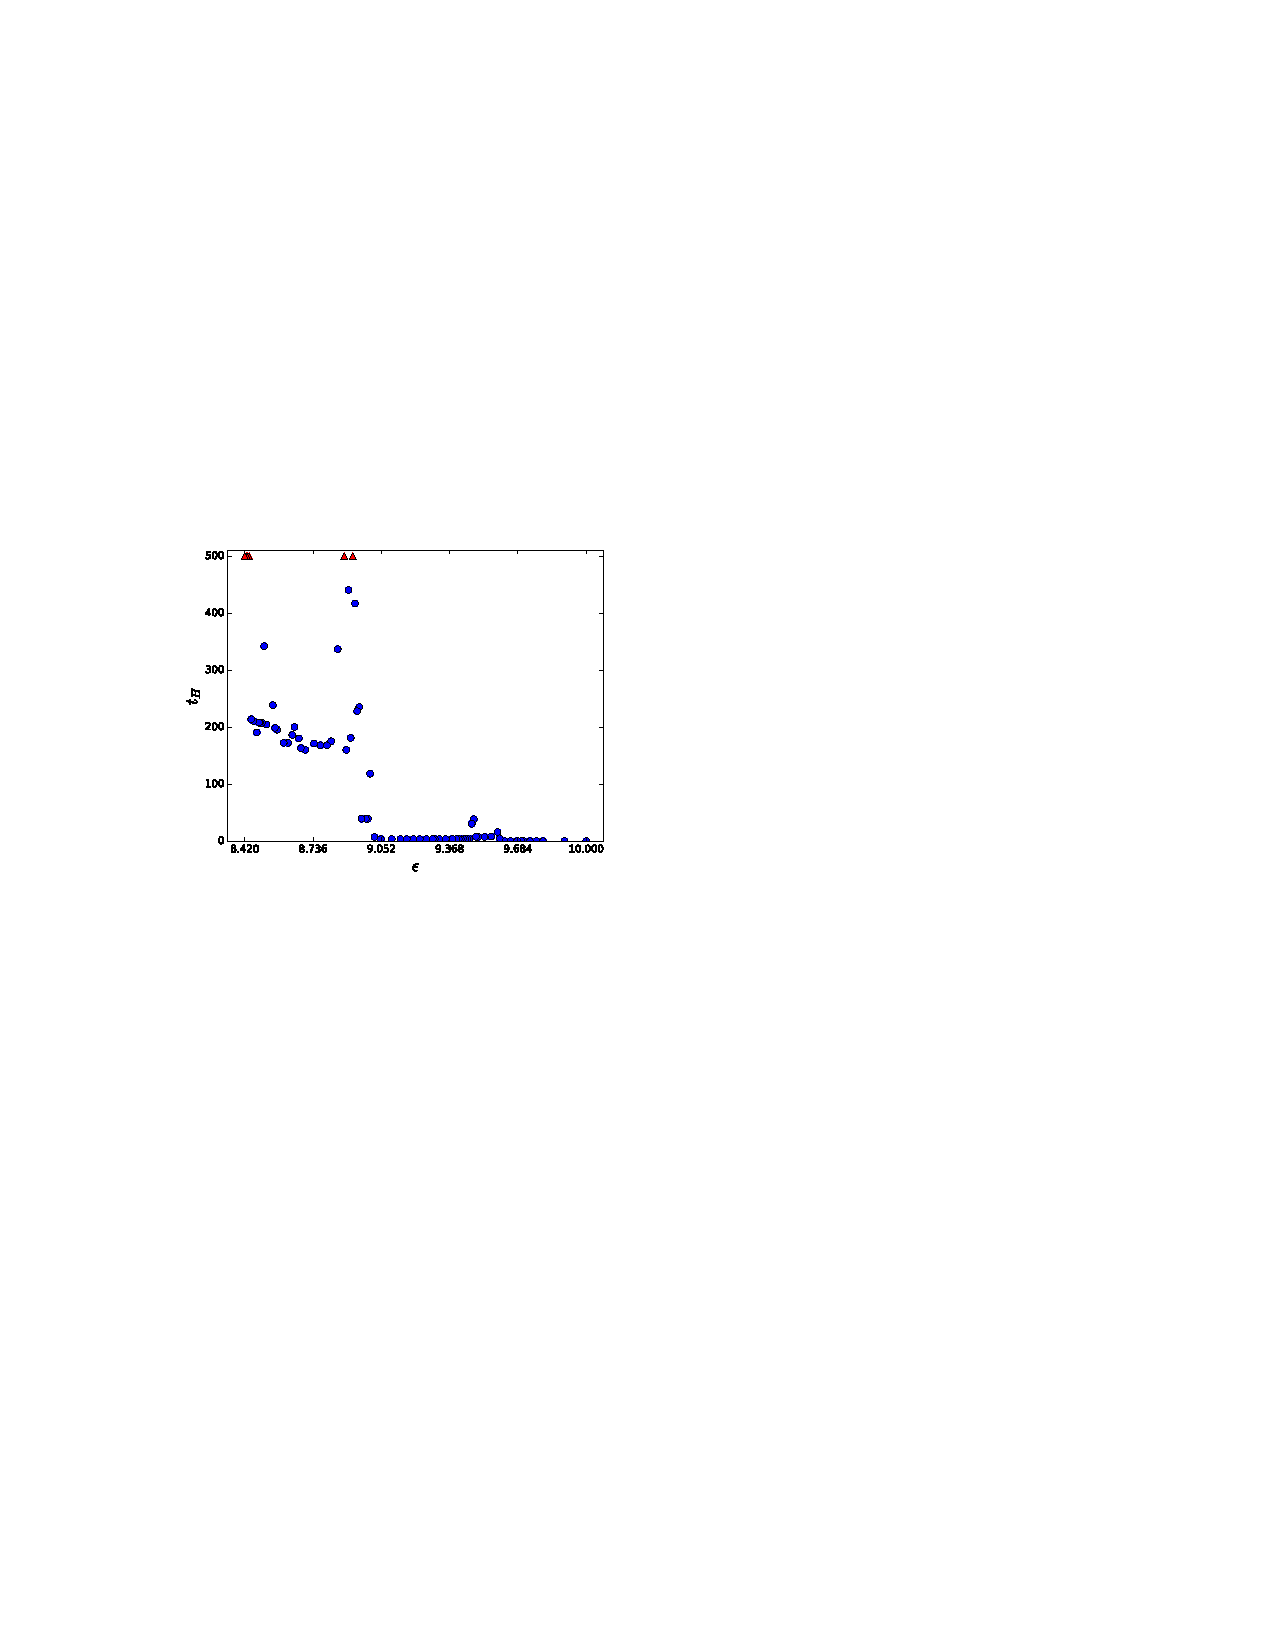
\includegraphics[width=\textwidth]{m20w016} \\ $\mu = 20$, $\sigma = 0.16$}
    \end{figure}
 \end{columns}
 \vfill
}

\frame
{
  \frametitle{Observations of Chaotic Behaviour}
  \begin{columns}
  \column{0.4\textwidth}
  \vspace{-0.35in}
  \bi
  \its Possible chaotic evolution $\to$ scalar self-interaction
  \its Previous chaotic evolution only seen in thin-shell interactions\footnotemark \: in AdS, scalar collapse in Gauss-Bonnet gravity\footnotemark
  \ei
  \column{0.6\textwidth}
      \begin{figure}
  	\centering
	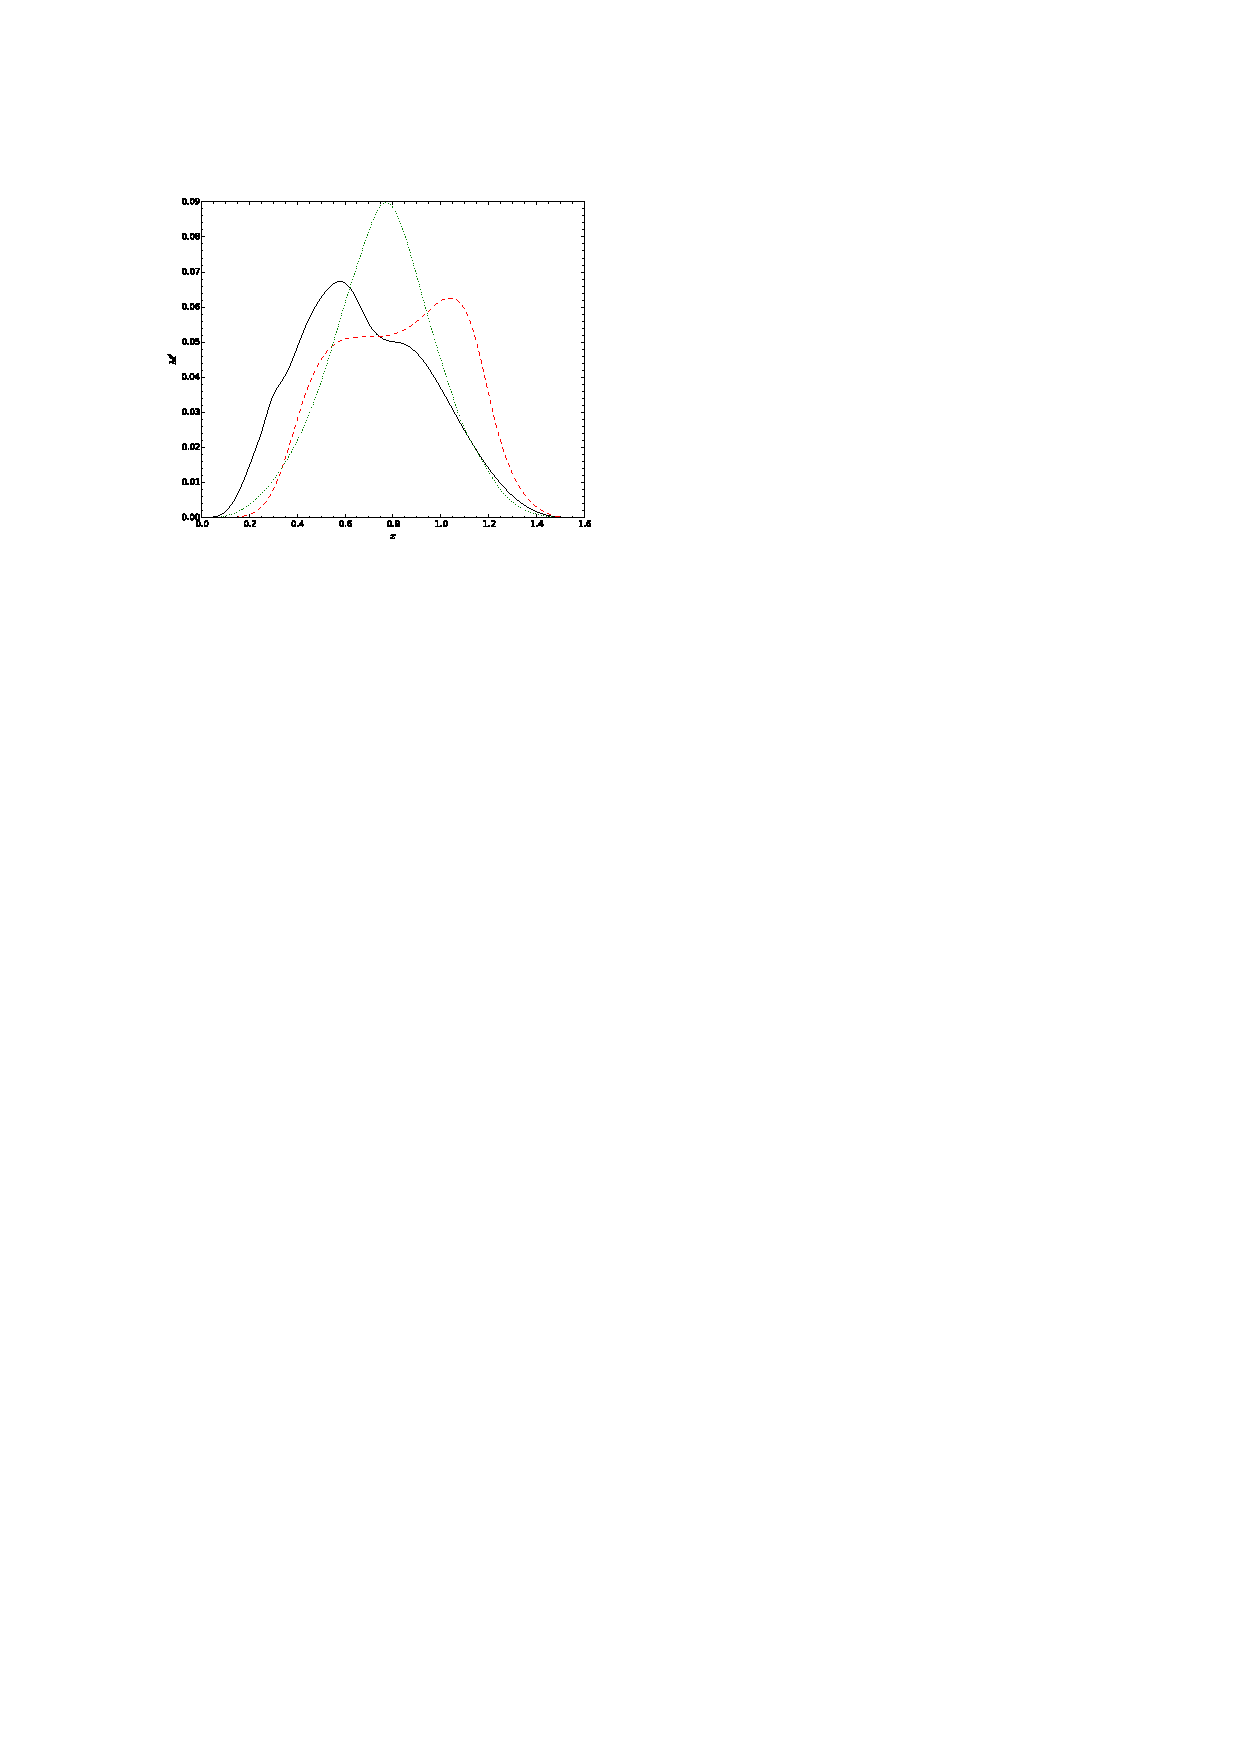
\includegraphics[width=\textwidth]{selfinteraction} 
	\vspace{-0.15in}
	\begin{align*} 
	\mu = 0,\; &\sigma=1.1, \; \epsilon = 1.01 \\ 
	&t = 60, {\color[rgb]{0.06,0.64,0.01} 62}, {\color[rgb]{.98,0,0.04} 64}
	\end{align*}
       \end{figure}
 \end{columns}
  \vspace{-0.4in}
 \footnotetext[5]{{\scr Brito {\it et al.} [1602.03535]}}
 \footnotetext[6]{{\scr Deppe, Kolly, {\it et al.} [1608.05402]}}

}

%%%%%%%%%%%%%%%%%%%%%%%%%%%%%%%%%%%%%%%%%%%%%%

\subsection{Phase Diagram}
\frame
{
  \frametitle{Phase Diagram}
  \uncover<2->{
  \bi
  \its {\color{orange} Unstable}, \uncover<3->{{\color[rgb]{.34,.69,0.29} metastable}, } \uncover<4->{{\color{red} irregular}, }\uncover<5->{and {\color{blue} stable} initial data}
  \ei 
  }
  \begin{figure}
  \centering
  \only<1>{
  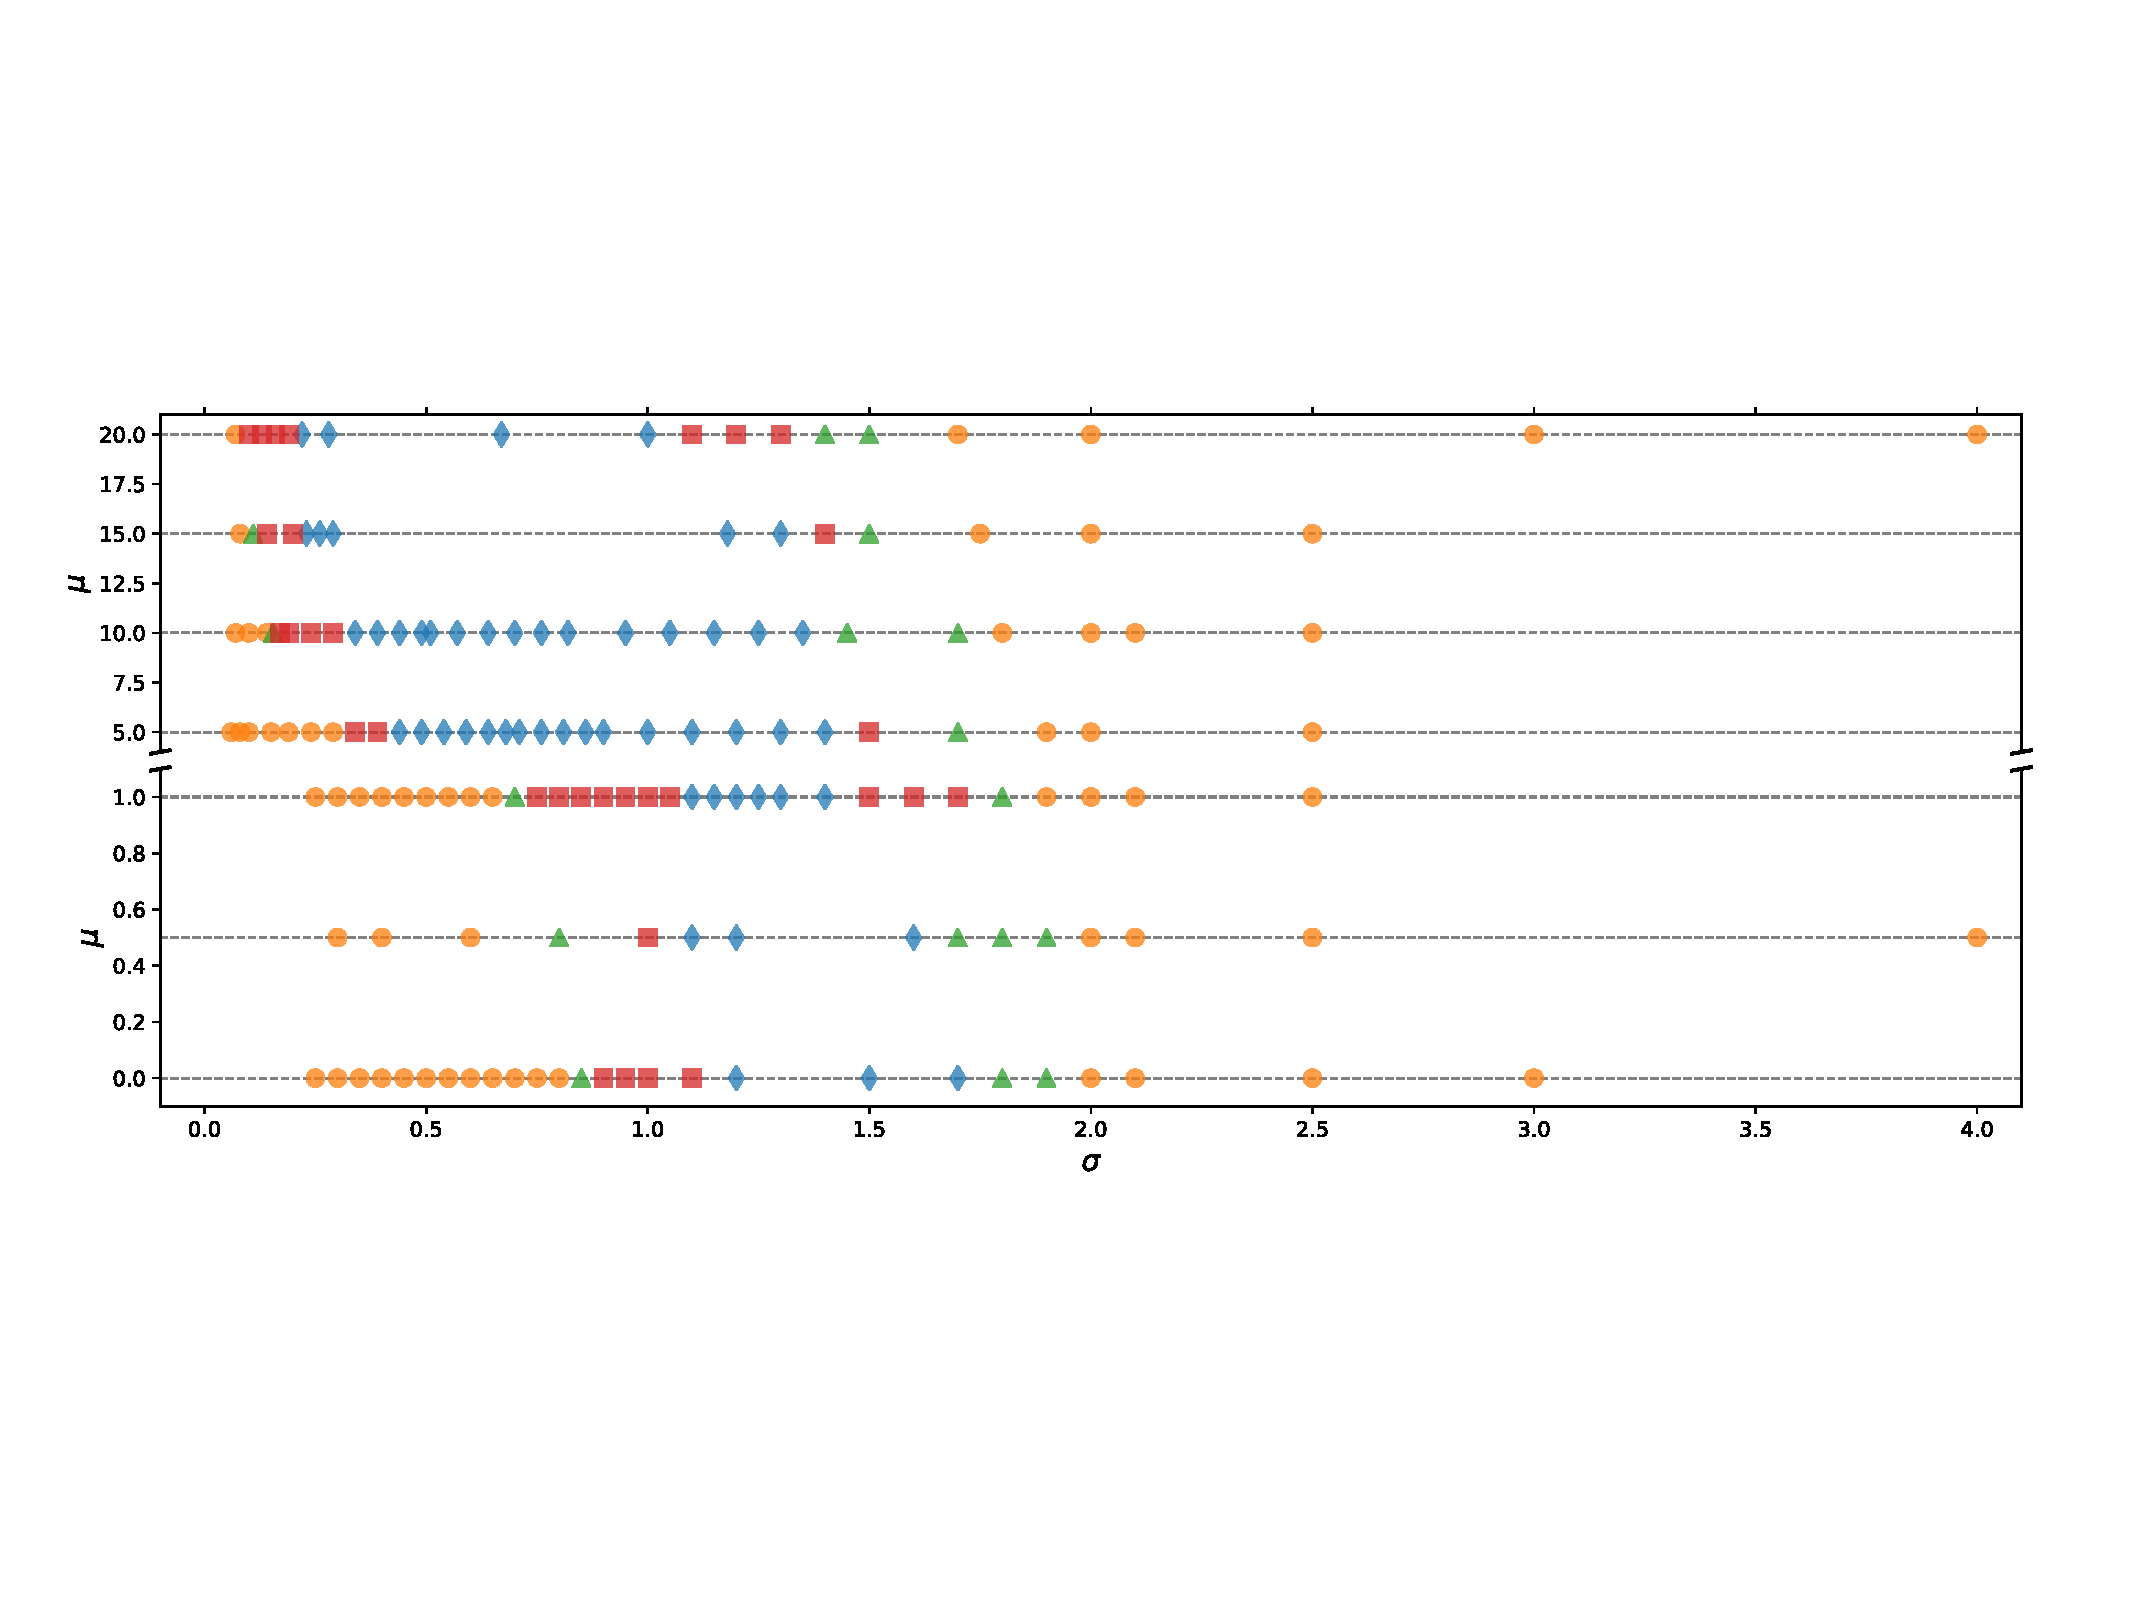
\includegraphics[width=\textwidth]{phase_plot}
  }
  \only<2>{
  \begin{center}
  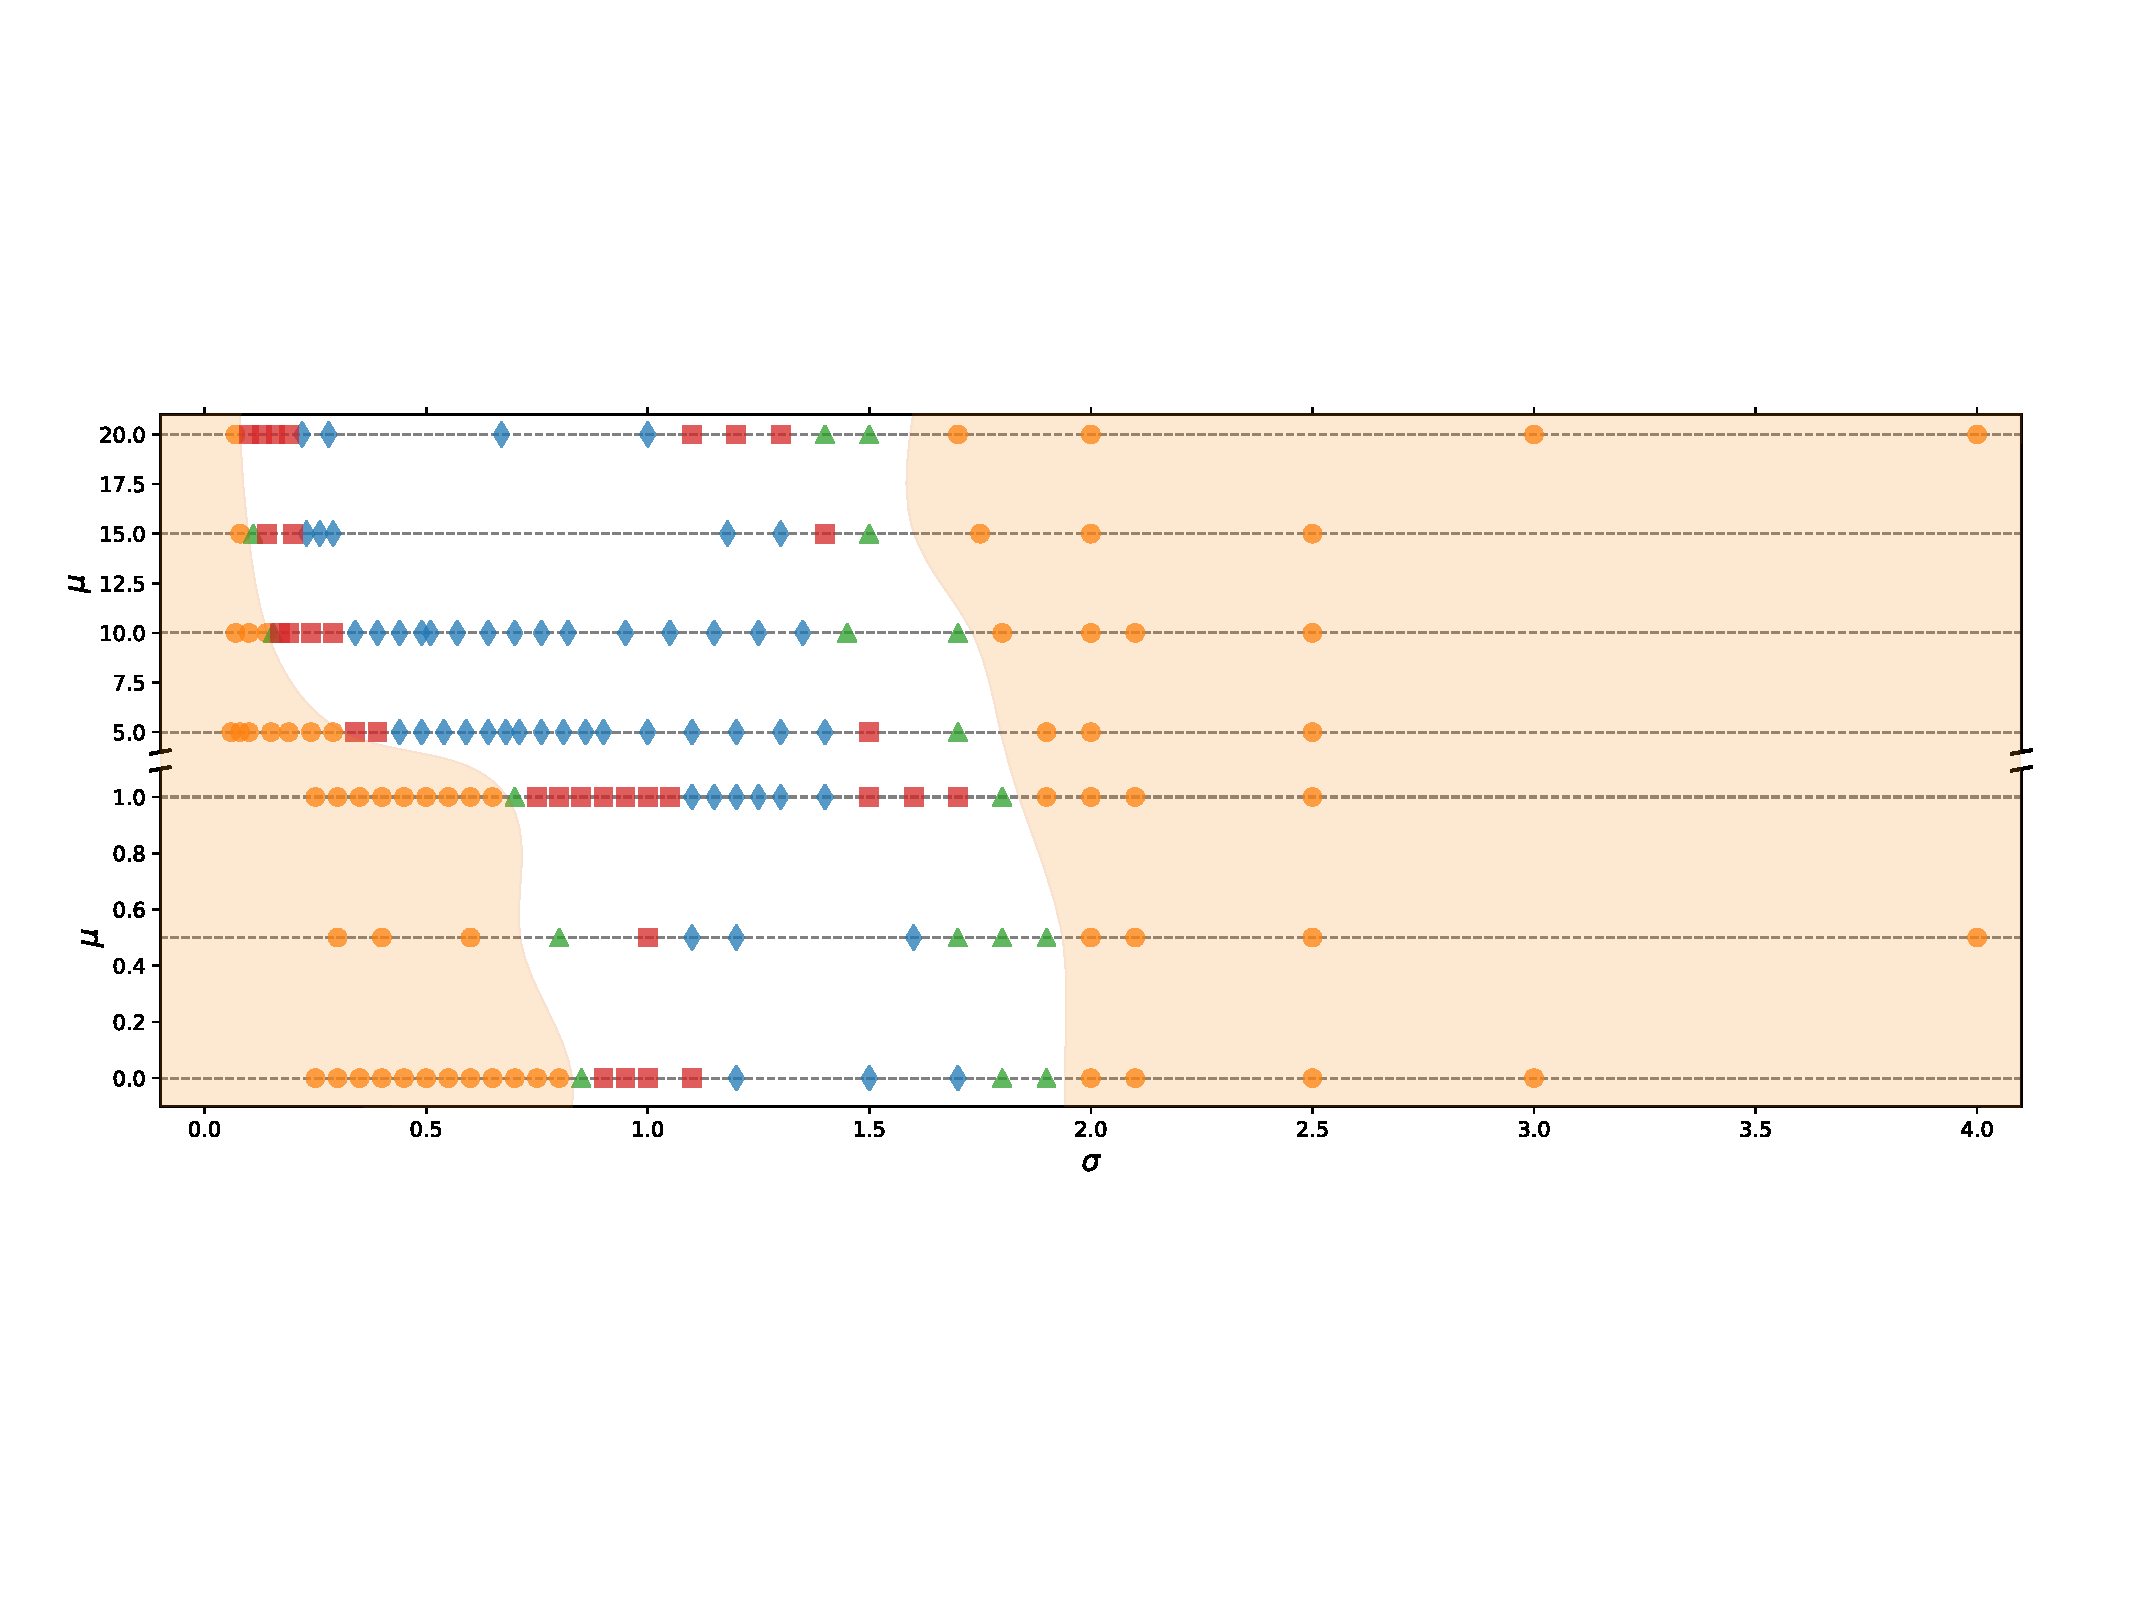
\includegraphics[width=\textwidth]{phase_sections1}
  \end{center}
  }
  \only<3>{
  \begin{center}
  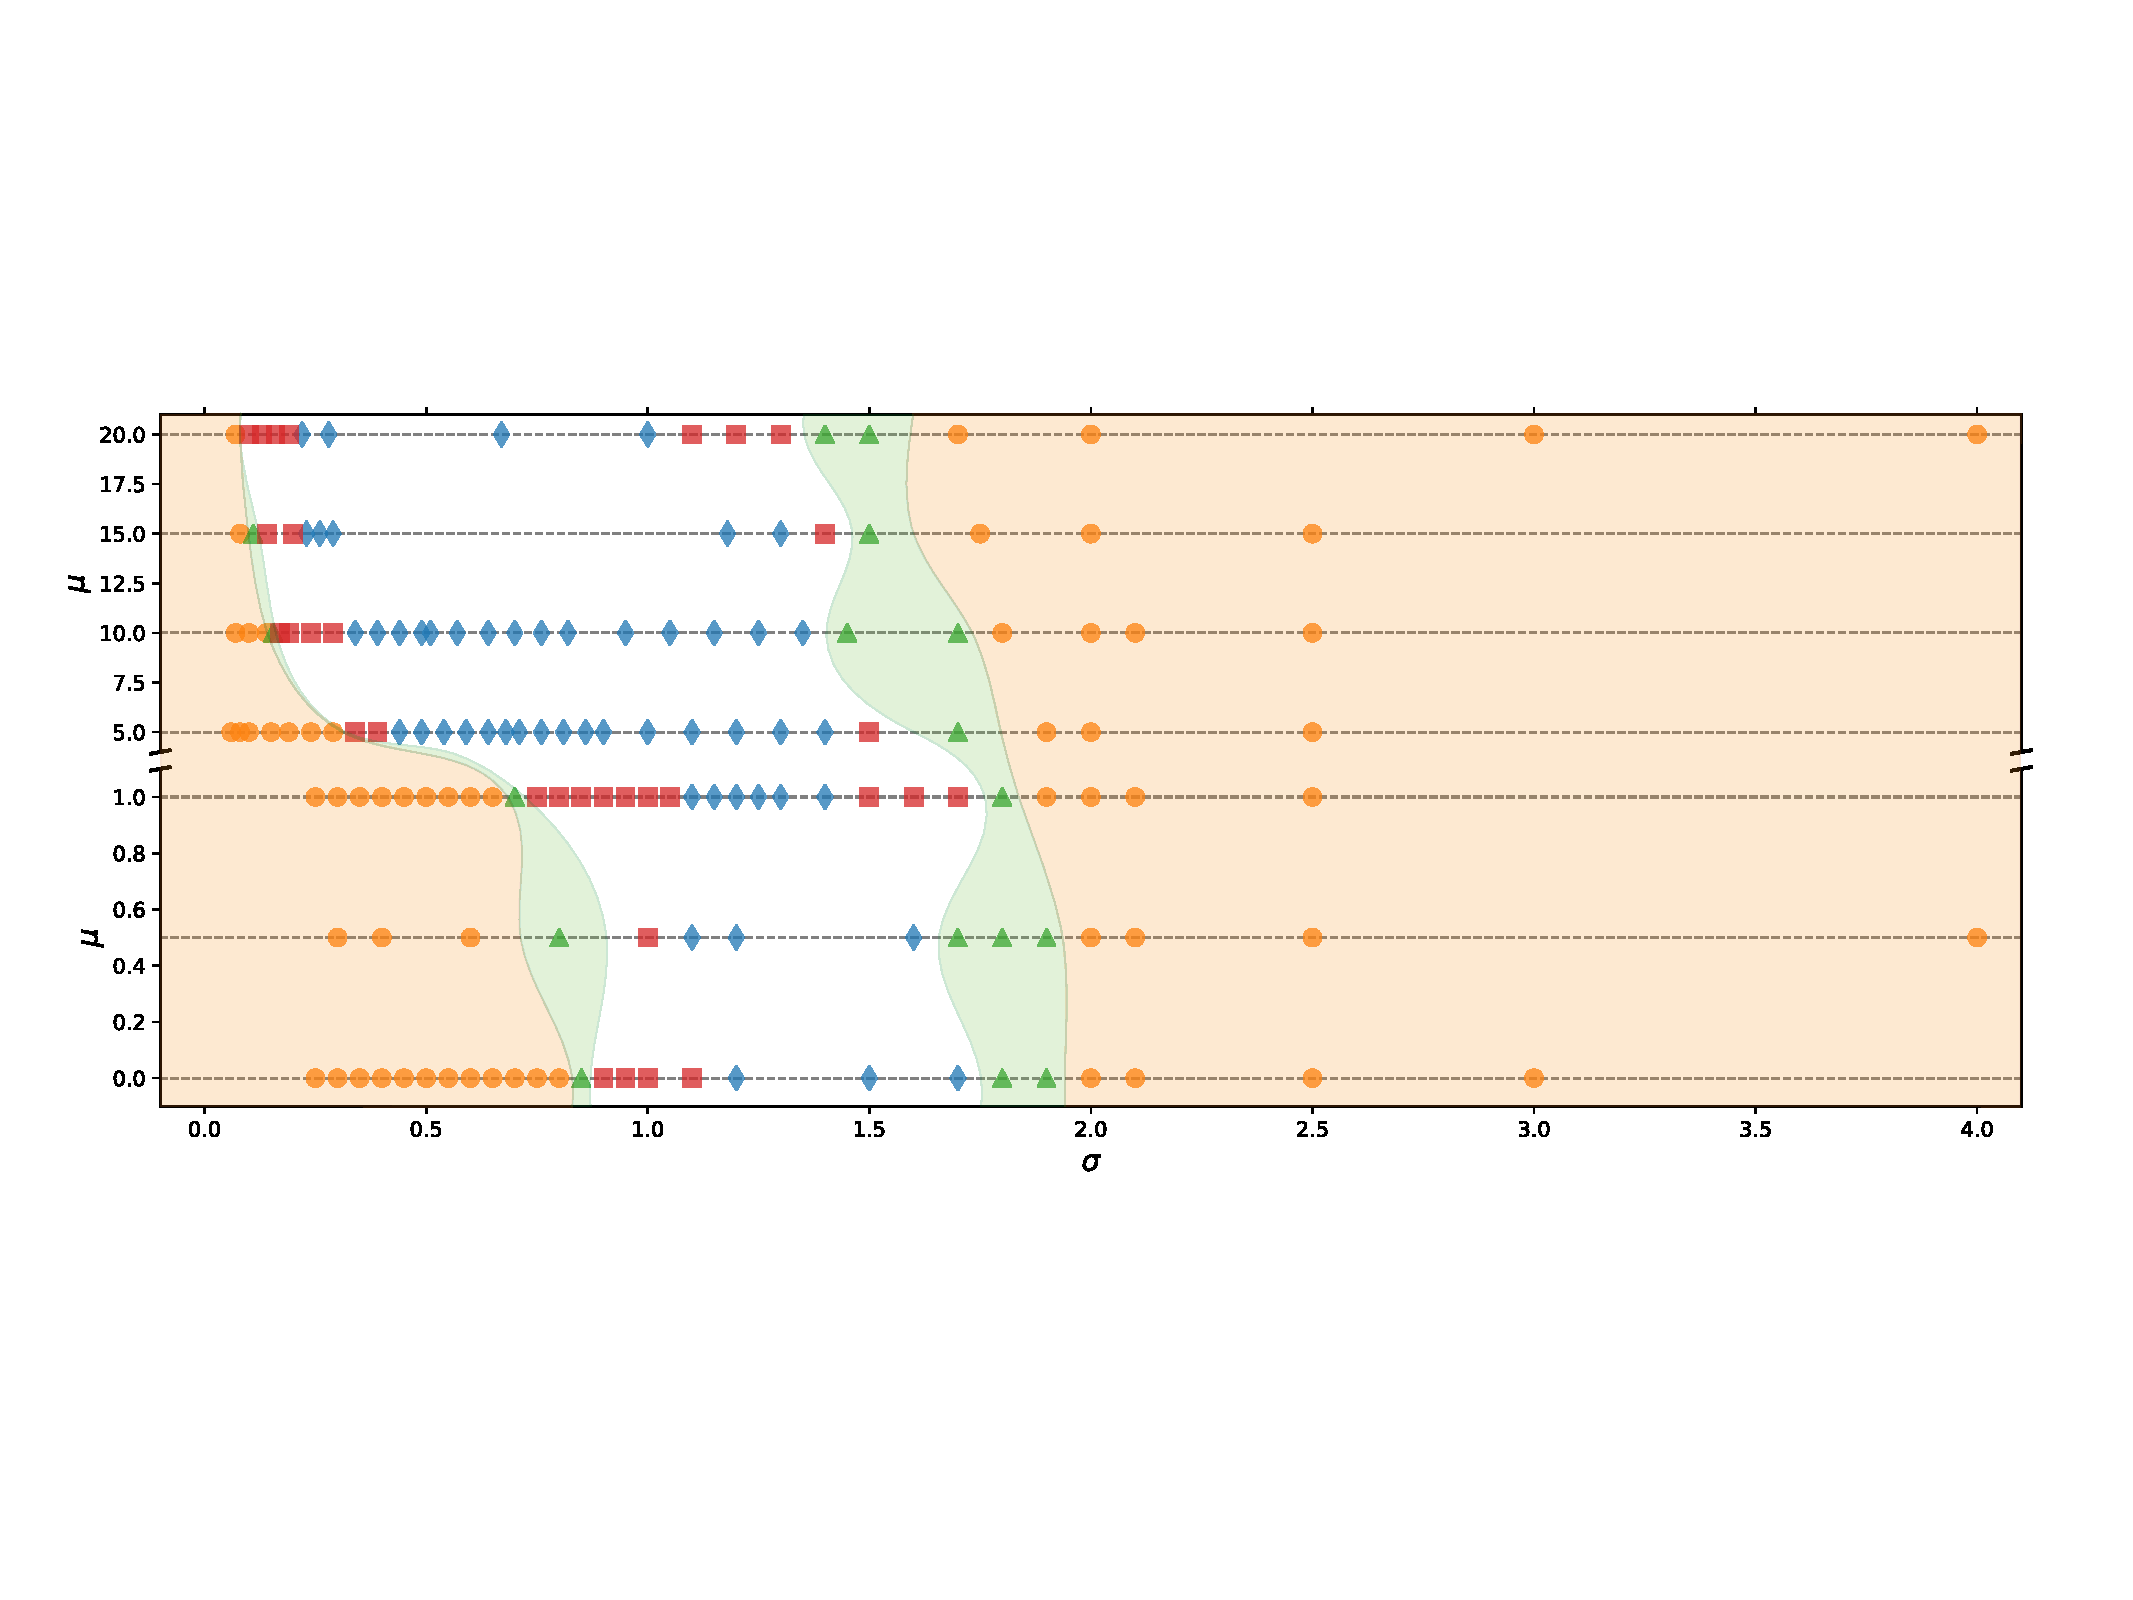
\includegraphics[width=\textwidth]{phase_sections2}
  \end{center}
  }
\only<4>{
  \begin{center}
  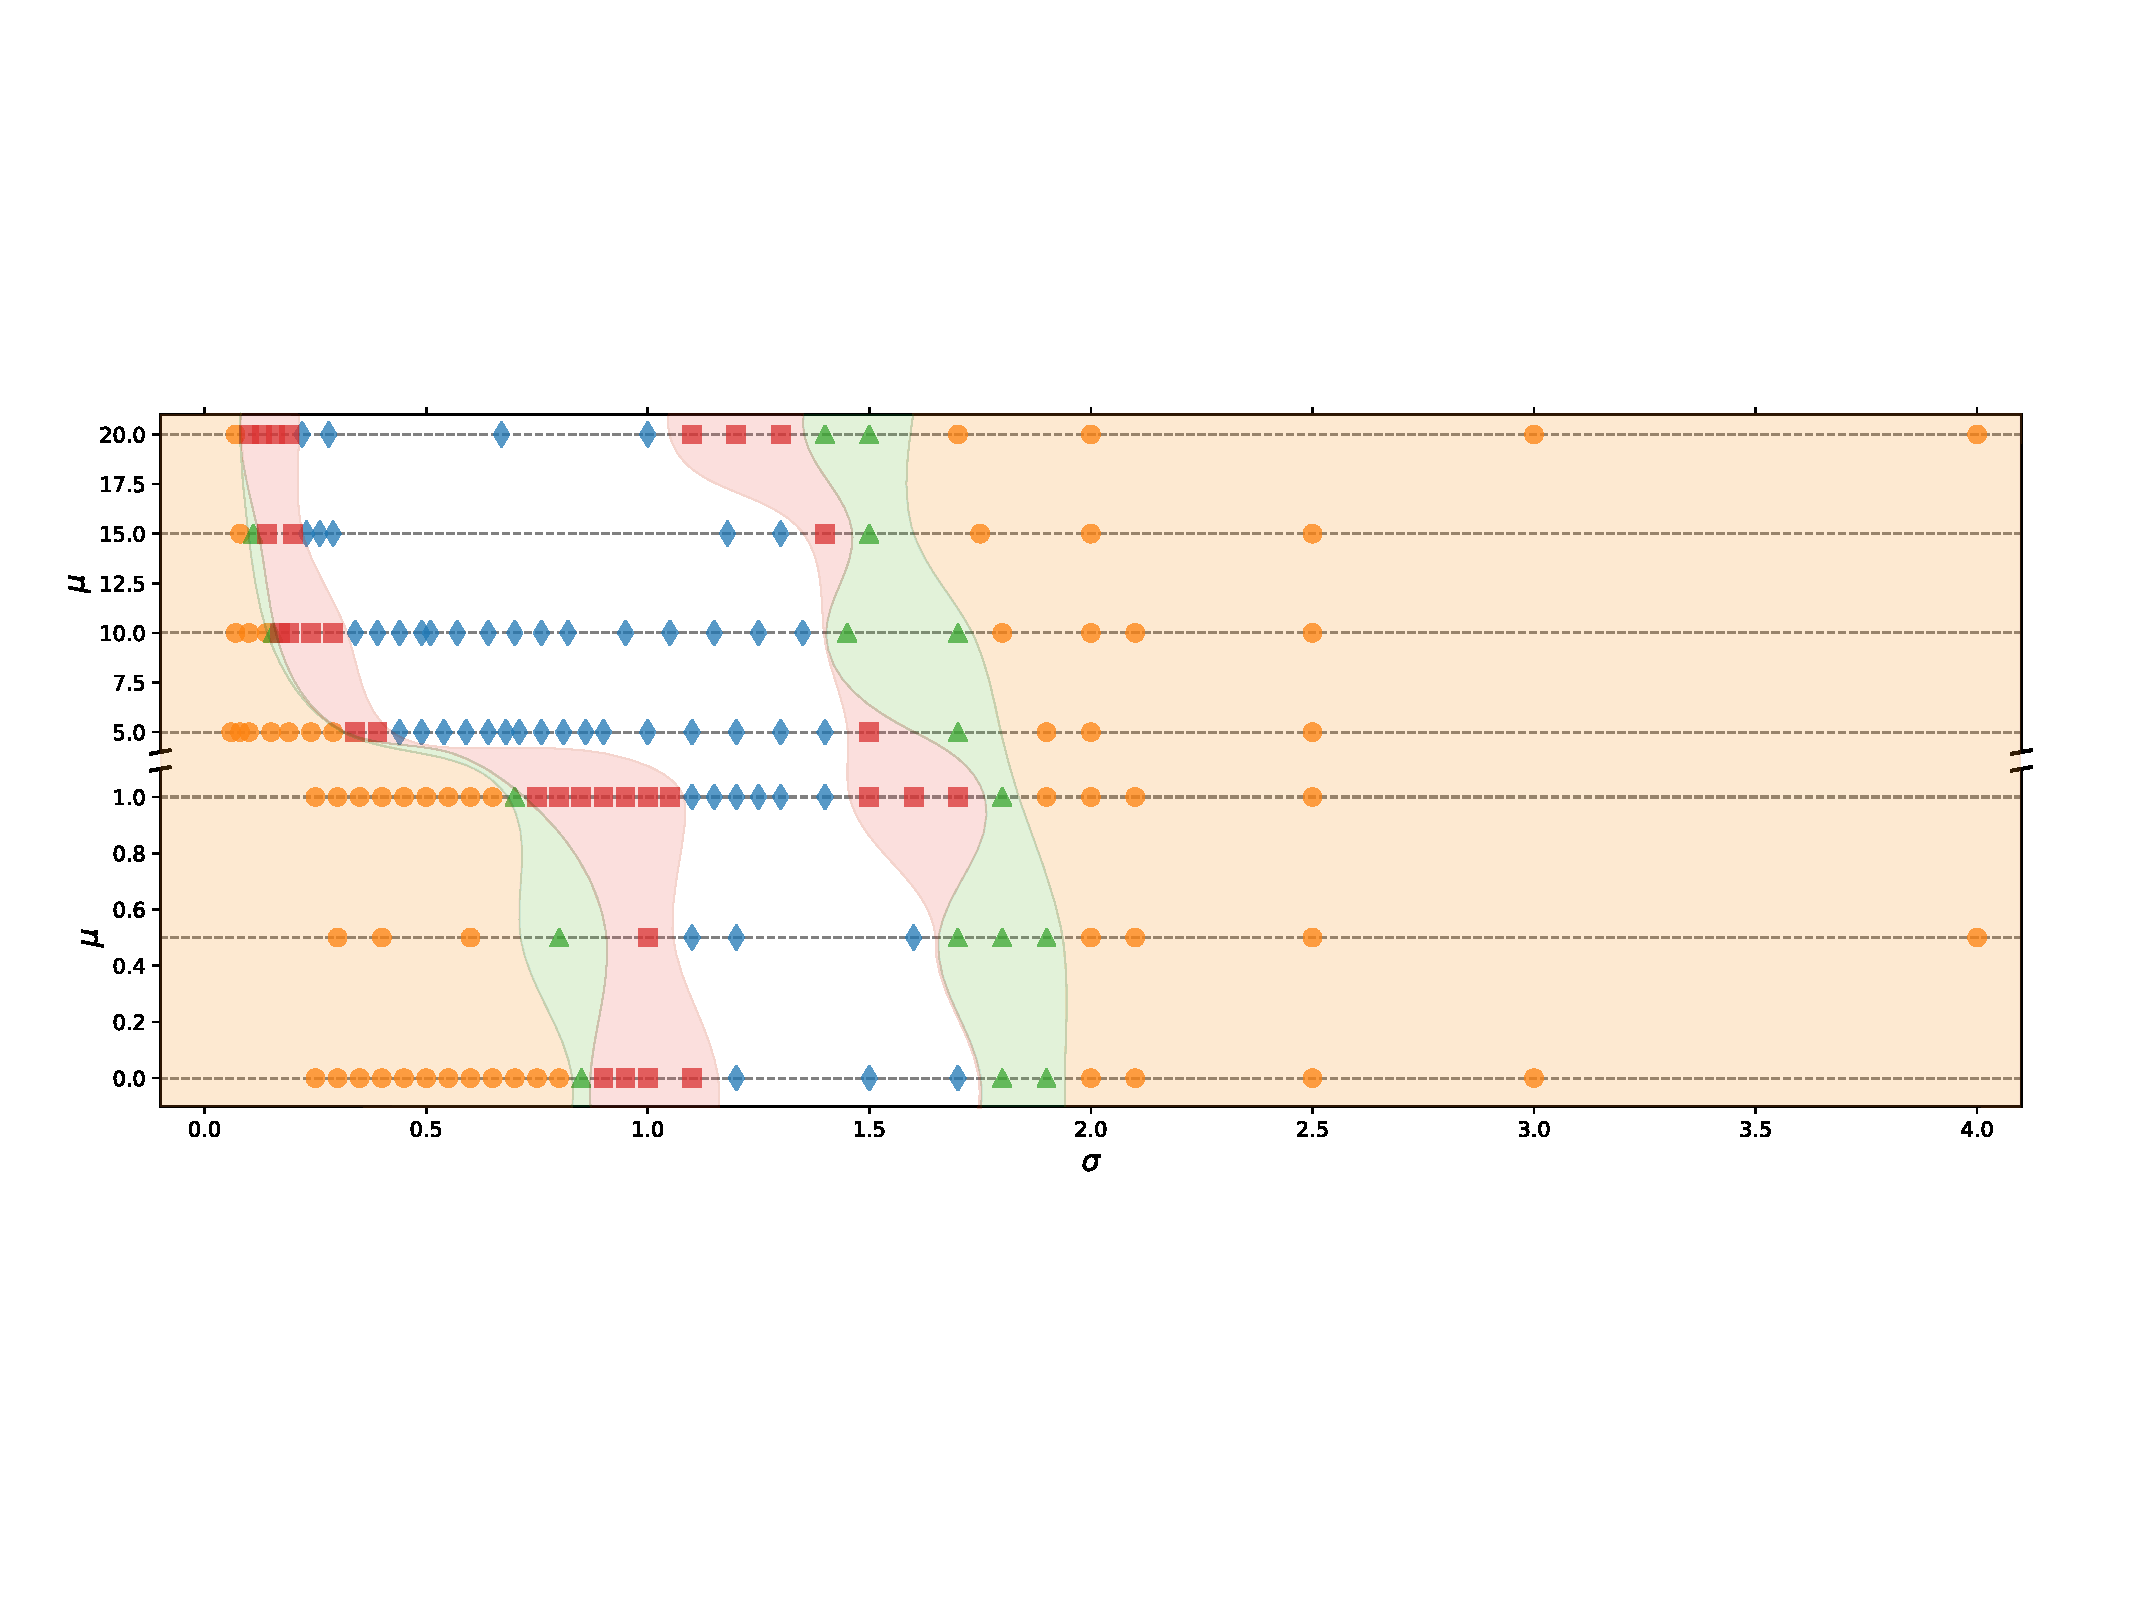
\includegraphics[width=\textwidth]{phase_sections3}
  \end{center}
  }
\only<5>{
  \begin{center}
  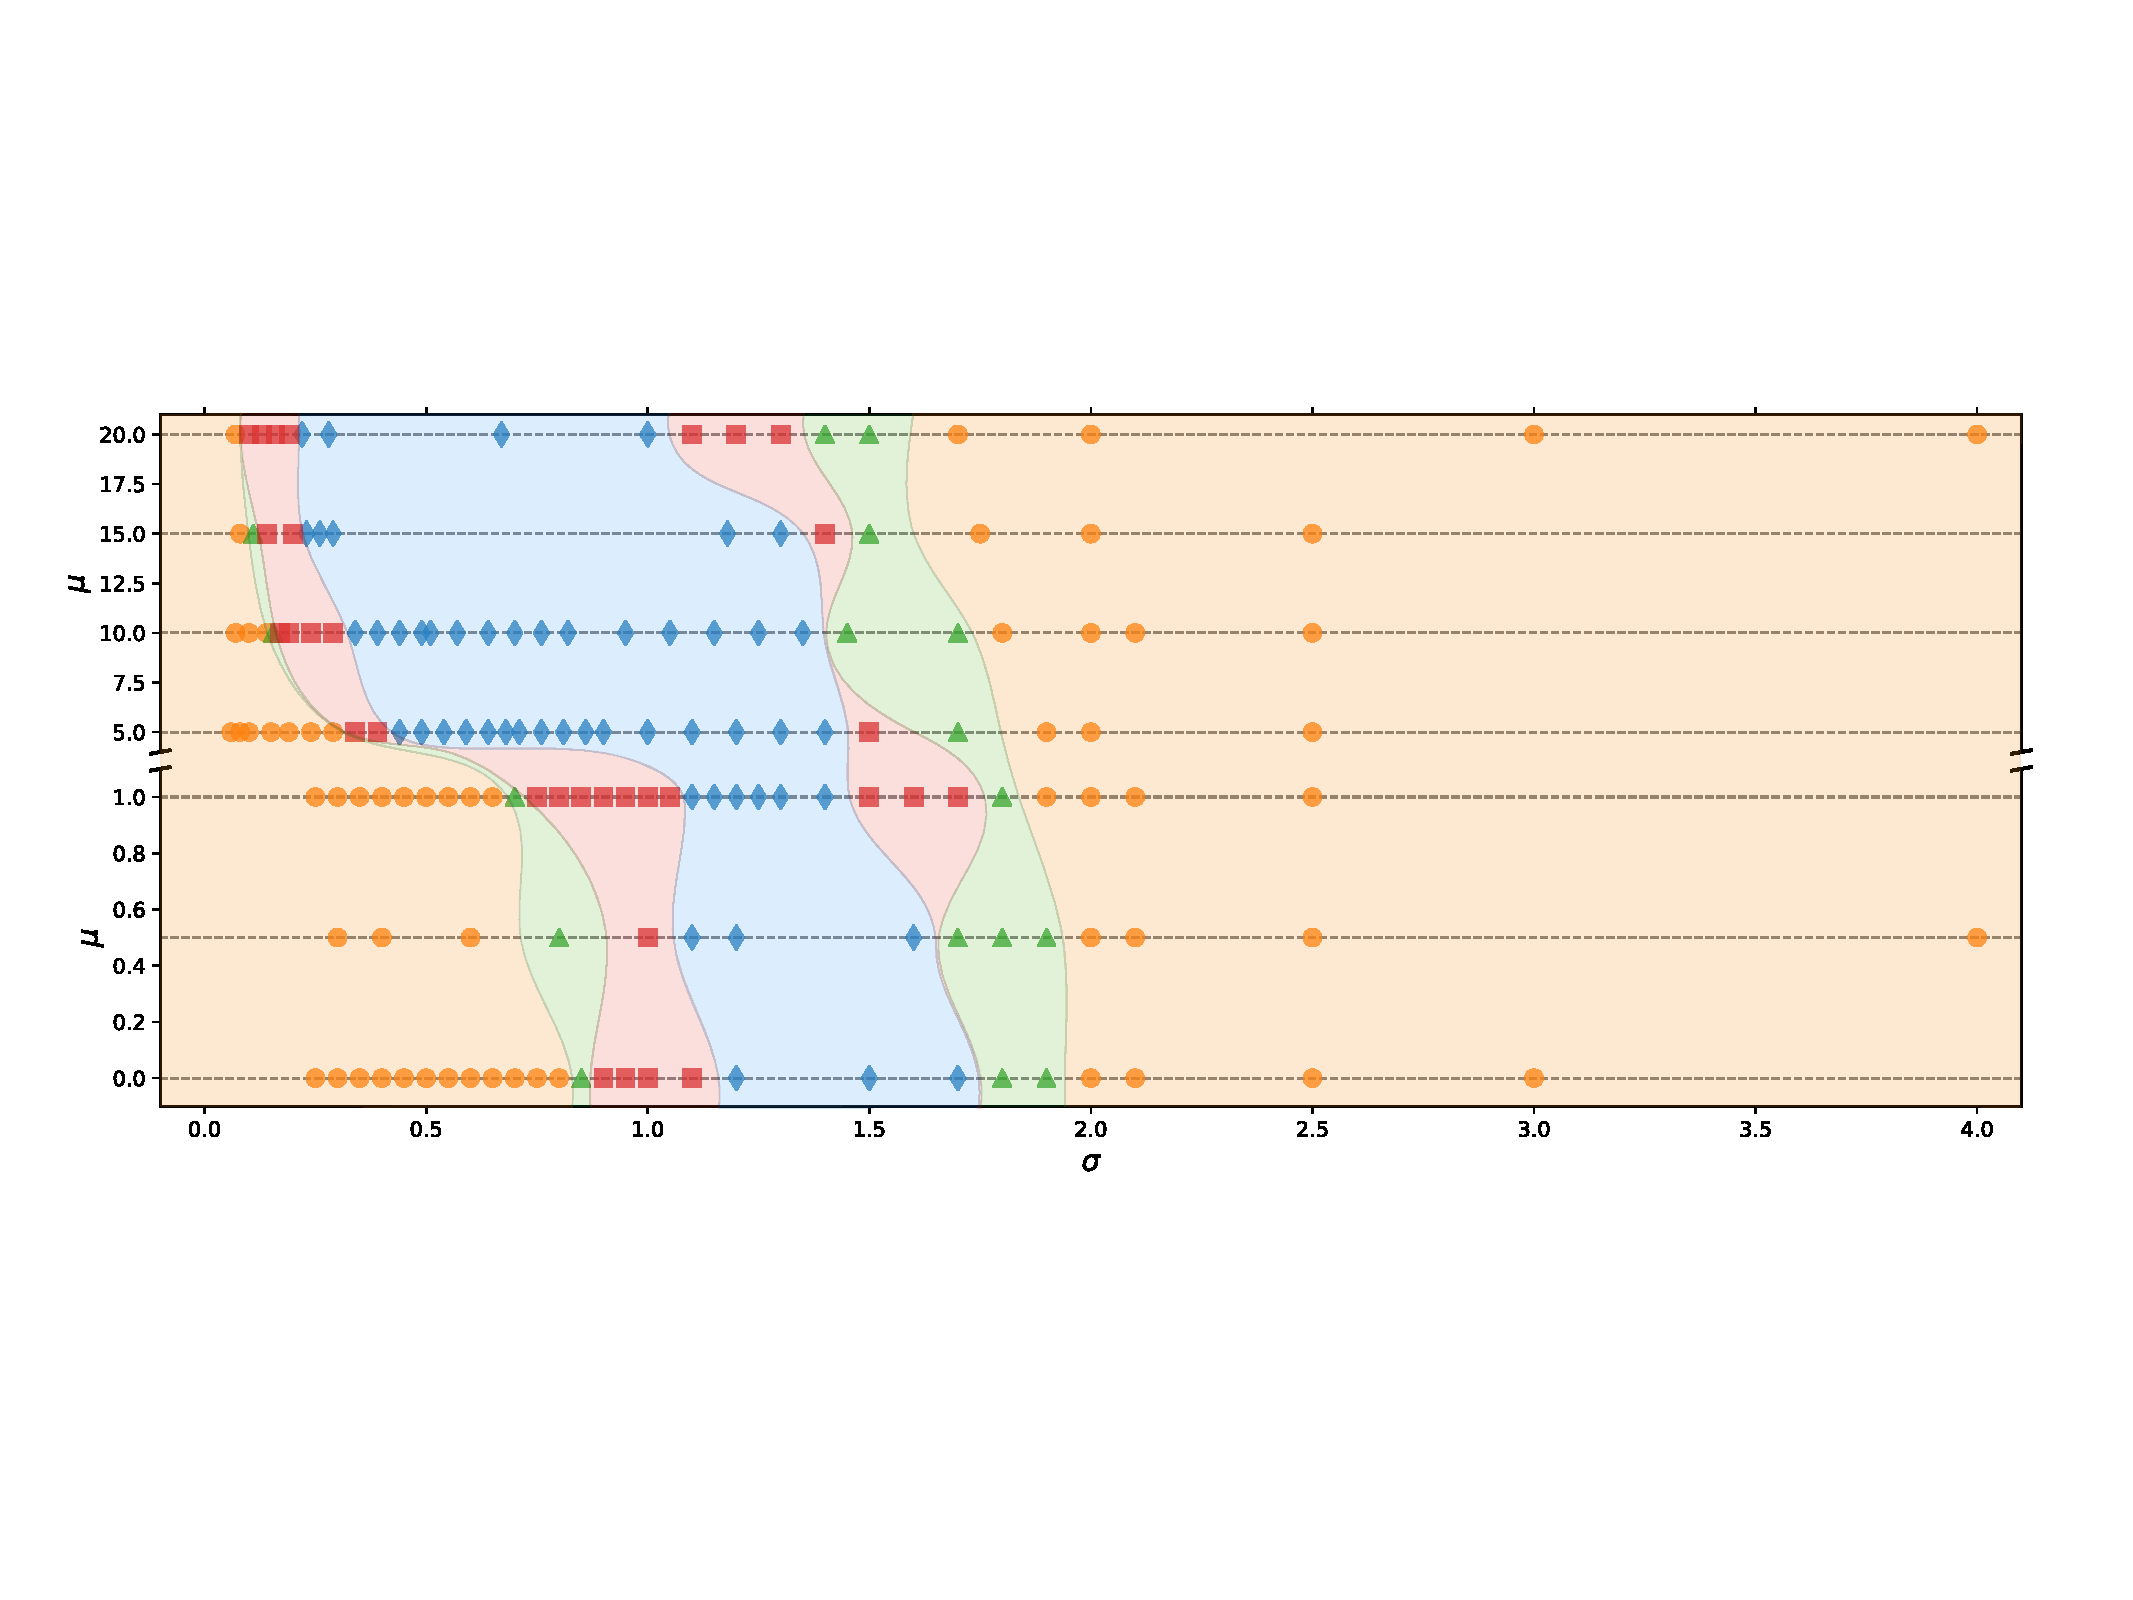
\includegraphics[width=\textwidth]{phase_sections4}
  \end{center}
  }
  \end{figure}
}

%\frame
%{
% \frametitle{Energy Cascades}
%  \bi
%  \its Stable solutions: \alert{direct} and \alert{inverse} energy cascades
%  \ei
%  \begin{columns}
%  \column{0.5\textwidth}
%      \begin{figure}
%      \centering
%      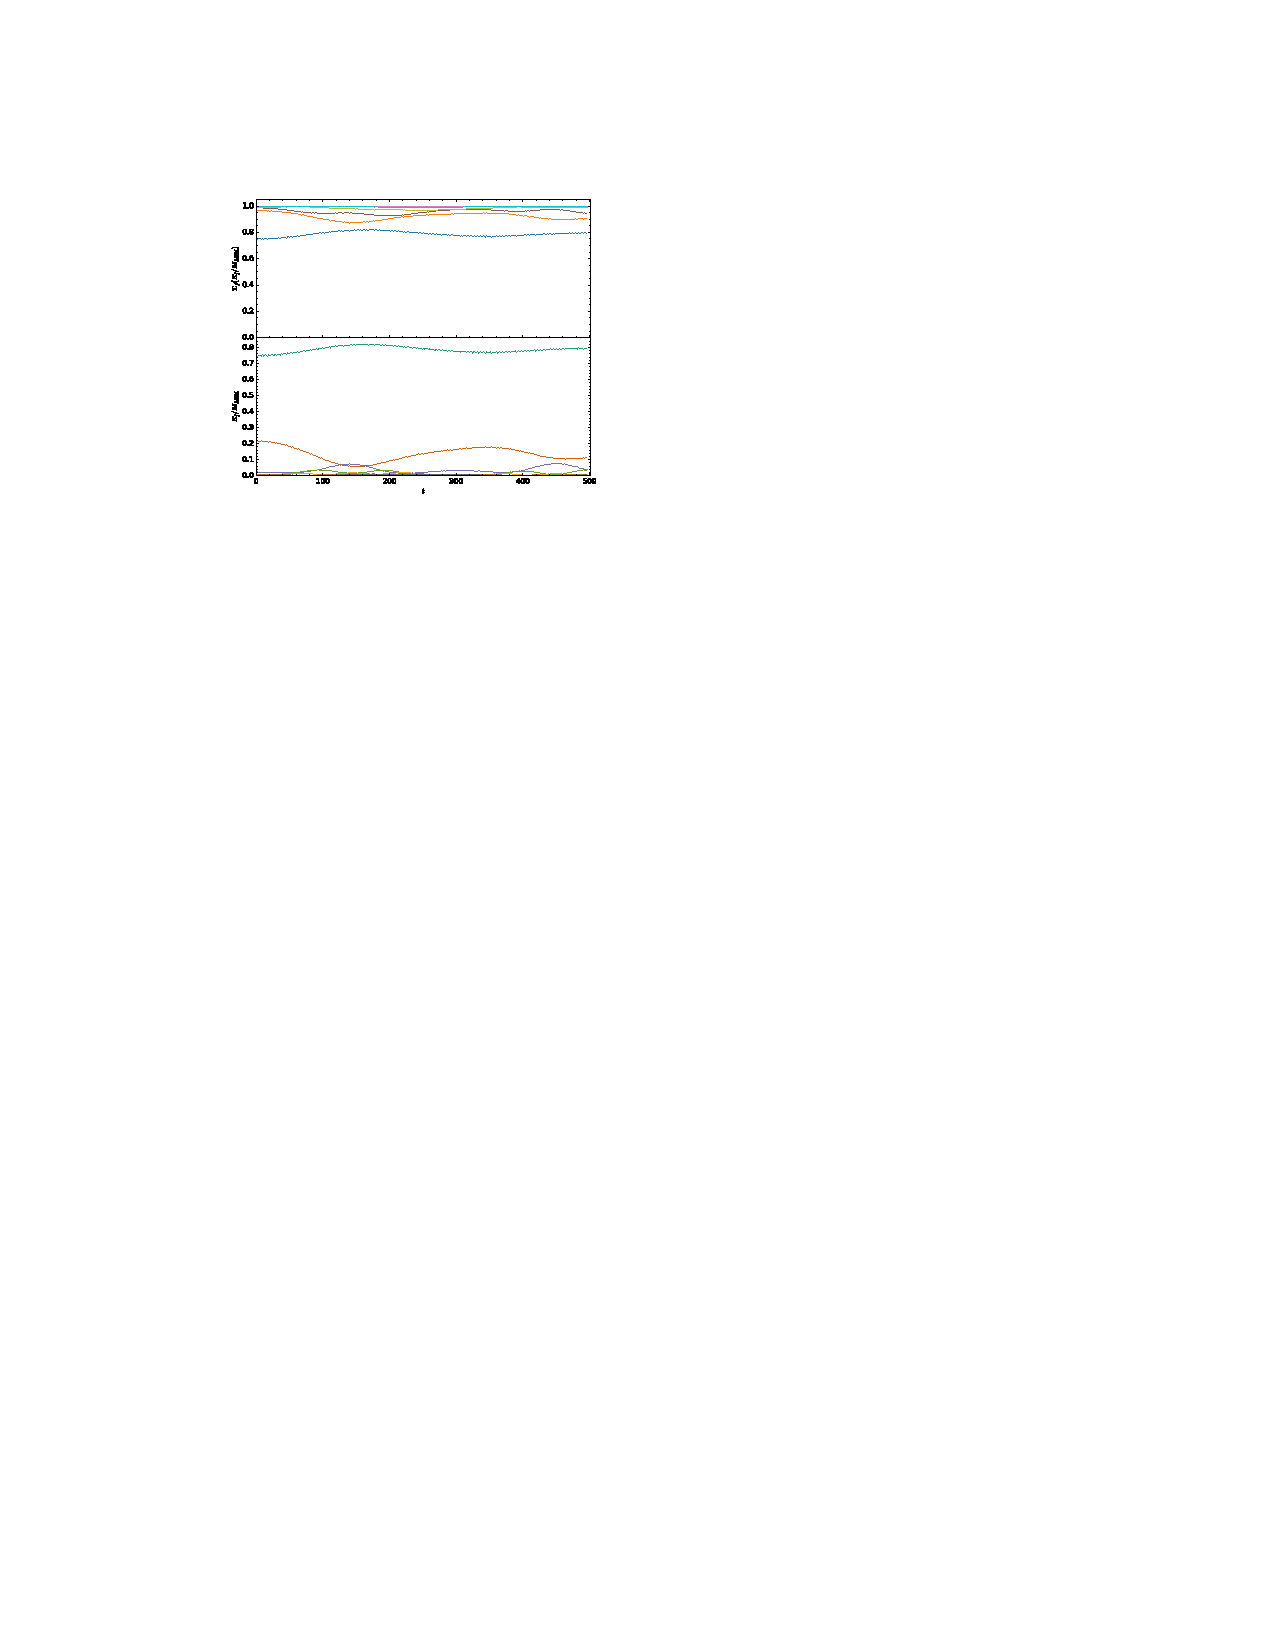
\includegraphics[width=\textwidth]{Em0w18} \\ $\mu = 0$, $\sigma = 1.8$, $\epsilon=0.13$ \\ Stable
%      \end{figure}
%  \column{0.5\textwidth}
%      \begin{figure}
%      \centering
%      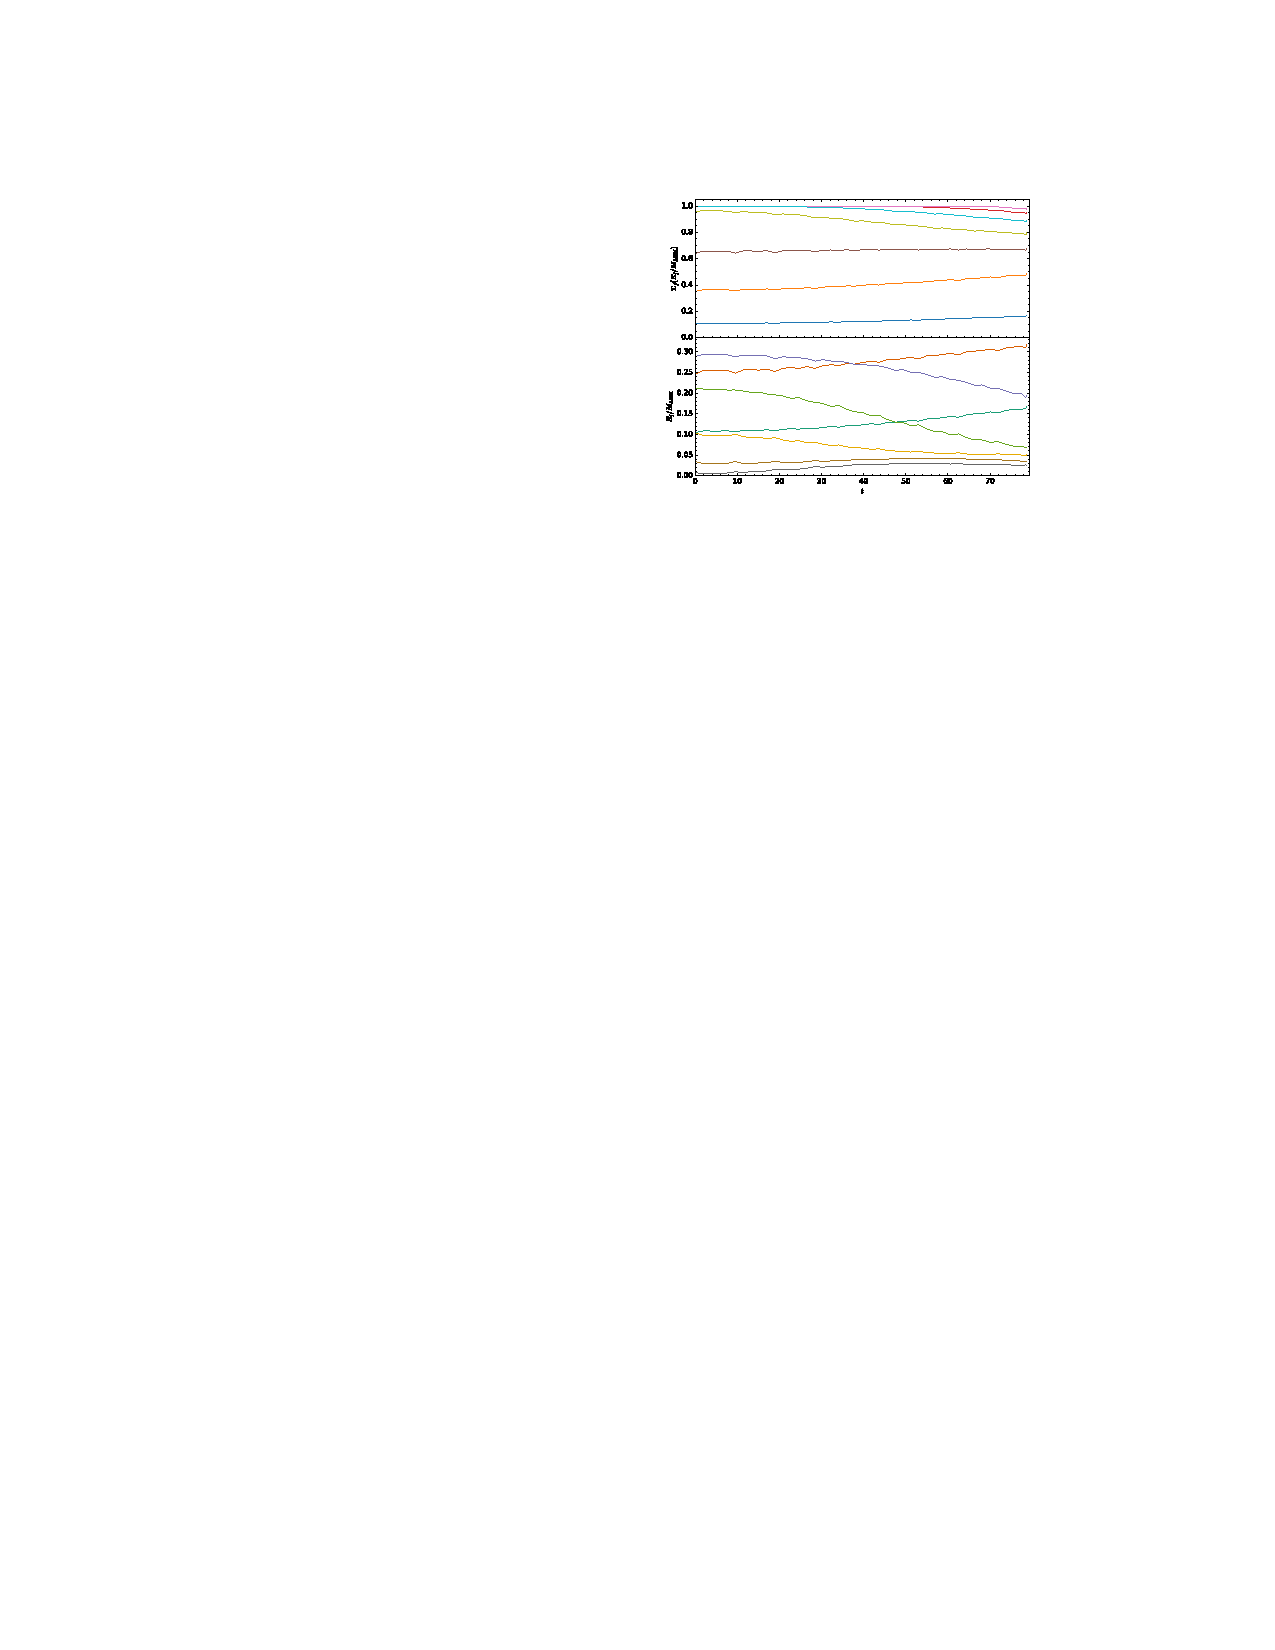
\includegraphics[width=\textwidth]{Em0w025} \\ $\mu = 0$, $\sigma = 0.25$, $\epsilon=2.28$ \\ Unstable
%      \end{figure}
%  \end{columns}
%}

\subsection*{}  
\frame
{
  \frametitle{Results}
  \bi
  \its First full phase diagram of stability in AdS$_5$ $\to$ islands of stability and ``shorelines''
  \its Evidence of metastable and irregular phases at finite $\epsilon$
  \its Fate of metastable phase as $\epsilon \to 0$ yet to be determined
  \its Irregular phase contains quasi-stable initial data\footnotemark$^{,}$\footnotemark $\to$ first evidence for weakly chaotic evolution in massless, spherically-symmetry scalars in AdS
  \its Metastable and irregular data to be studied in multiscale perturbation theory
  \ei
  
  \footnotetext[7]{{\scr Deppe \& Frey [1508.02709]}}
  \footnotetext[8]{{\scr Buchel {\it et al.} [1304.4166]}}
}  
  
%%%%%%%%%%%%%%%%%%%%%%%%%%%%%%%%%%%%%%%%%%%%%%
%%%%%%%%%%%%%%%%%%%%%%%%%%%%%%%%%%%%%%%%%%%%%%

\section{High-Temperature QP Solutions in AdS$_4$}
\frame[c, noframenumbering]
{
  \frametitle{}
  \begin{center}
    \begin{mybox}[]
    B Cownden, N Deppe, and AR Frey, {\it On the Stability of High-Temperature, Quasi-Periodic Solutions for Massless Scalars in AdS$_4$}, In progress.
    \end{mybox}
  \end{center}
}

%%%%%%%%%%%%%%%%%%%%%%%%%%%%%%%%%%%%%%%%%%%%%%

\subsection{The Two-Time Formalism (TTF)}
\frame
{
  \frametitle{The Two-Time Formalism (TTF)}
  \bi
  \its Small perturbations in AdS$_4$: expand scalar field, metric functions in $\epsilon$
  \its $\mc O(\epsilon)$: $\phi_1$ in terms of eigenfunctions of AdS, \alert<1>{$e_j(x)$}
  \its Integer eigenvalues $\omega_j = (2j + d)$ $\to$ fully resonant spectrum
  \its<2->{Secular growth of resonant contributions $\to$ scalar field collapse}
  \its <2->{$\mc O(\epsilon^3)$: \alert{source term} for resonant contributions}
  \its <2->{Complex amplitudes vary with ``slow time'' $\tau$ $\to$ flow equation to absorb resonances\footnote<2->{{\scr Balasubramanian {\it et al.} [1403.6471]}}}
  \ei
  \vfill
  \begin{overlayarea}{\textwidth}{0.3\textheight}
  \begin{align*}
  \only<1>{
  \phi_1 (t,x) = \sum^\infty_{j=0} \Big( A_j(t) e^{i\omega_j t} + \bar A_j (t) e^{-i \omega_j t} \Big) \: \alert{e_j (x)}
  }
  \only<2>{
   -2i \omega_\ell \frac{d A_\ell (\tau)}{d \tau} &= \sum_{i,j,k} \alert{f^{(\ell)}_{ijk}} \bar A_i A_j A_k
  }
  \end{align*}
  \end{overlayarea}

}

%%%%%%%%%%%%%%%%%%%%%%%%%%%%%%%%%%%%%%%%%%%%%%

\subsection{Quasi-Periodic Solutions}
\frame
{
  \frametitle{Quasi-Periodic Solutions I}
  \bi 
  \its Renormalization flow techniques to cancel an infinite number of resonances $\to$ express non-vanishing ones analytically\footnote<1->{{\scr Craps {\it et al.} [1407.6273]}}
  \its Need to truncate number of modes to find solutions: $\jm < \infty$ (must be robust as $\jm \to \infty$)
  \its<2->{Quasi-periodic\footnote<2->{{\scr Balasubramanian {\it et al.} [1403.6471]}} solutions $A_j = \alpha_j e^{i \beta_j \tau}$ with ${\alpha_j, \beta_j \in \mathbb{R}}$ $\to$ TTF equations become time-independent when $\beta_j = \beta_0 + j(\beta_1 - \beta_0)$}
  \its<2->{TTF: conserved quantities\footnote<2->{{\scr Craps {\it et al.} [1412.3249]}} $(E, N)$ $\to$ classify solutions by $T \equiv E/N$}
  \its<2->{Solve QP equation using Newton-Raphson method}
  \ei
  \vspace{-0.15in}
  \begin{overlayarea}{\textwidth}{0.2\textheight}
   \begin{align*}
   \uncover<2->{
  2\omega_\ell \alpha_\ell \beta_\ell = T_\ell \alpha_\ell^3 + \sum_{i \neq \ell} R_{i\ell} \alpha_i^2 \alpha_\ell + \stackrel{\ell \leq i + j}{\sum_{i \neq \ell} \sum_{j \neq \ell}} S_{i j (i+j-\ell)\ell} \alpha_i \alpha_j \alpha_{i+j-\ell}
  }
  \end{align*}
  \end{overlayarea}
}

\frame
{
  \frametitle{Quasi-Periodic Solutions II}
  \begin{columns}
  \column{0.3\textwidth}
  \bi
  \its Solutions found for $3 \leq T \lesssim 5.5$
  \its<2->{Able to extend existing solutions from $\jm \sim 100$ to $\jm = 500$}
  \its<2->{Robust in $\jm \to \infty$ limit}
  \ei
  \column{0.7\textwidth}
  \begin{figure}
  \centering
    \only<1>{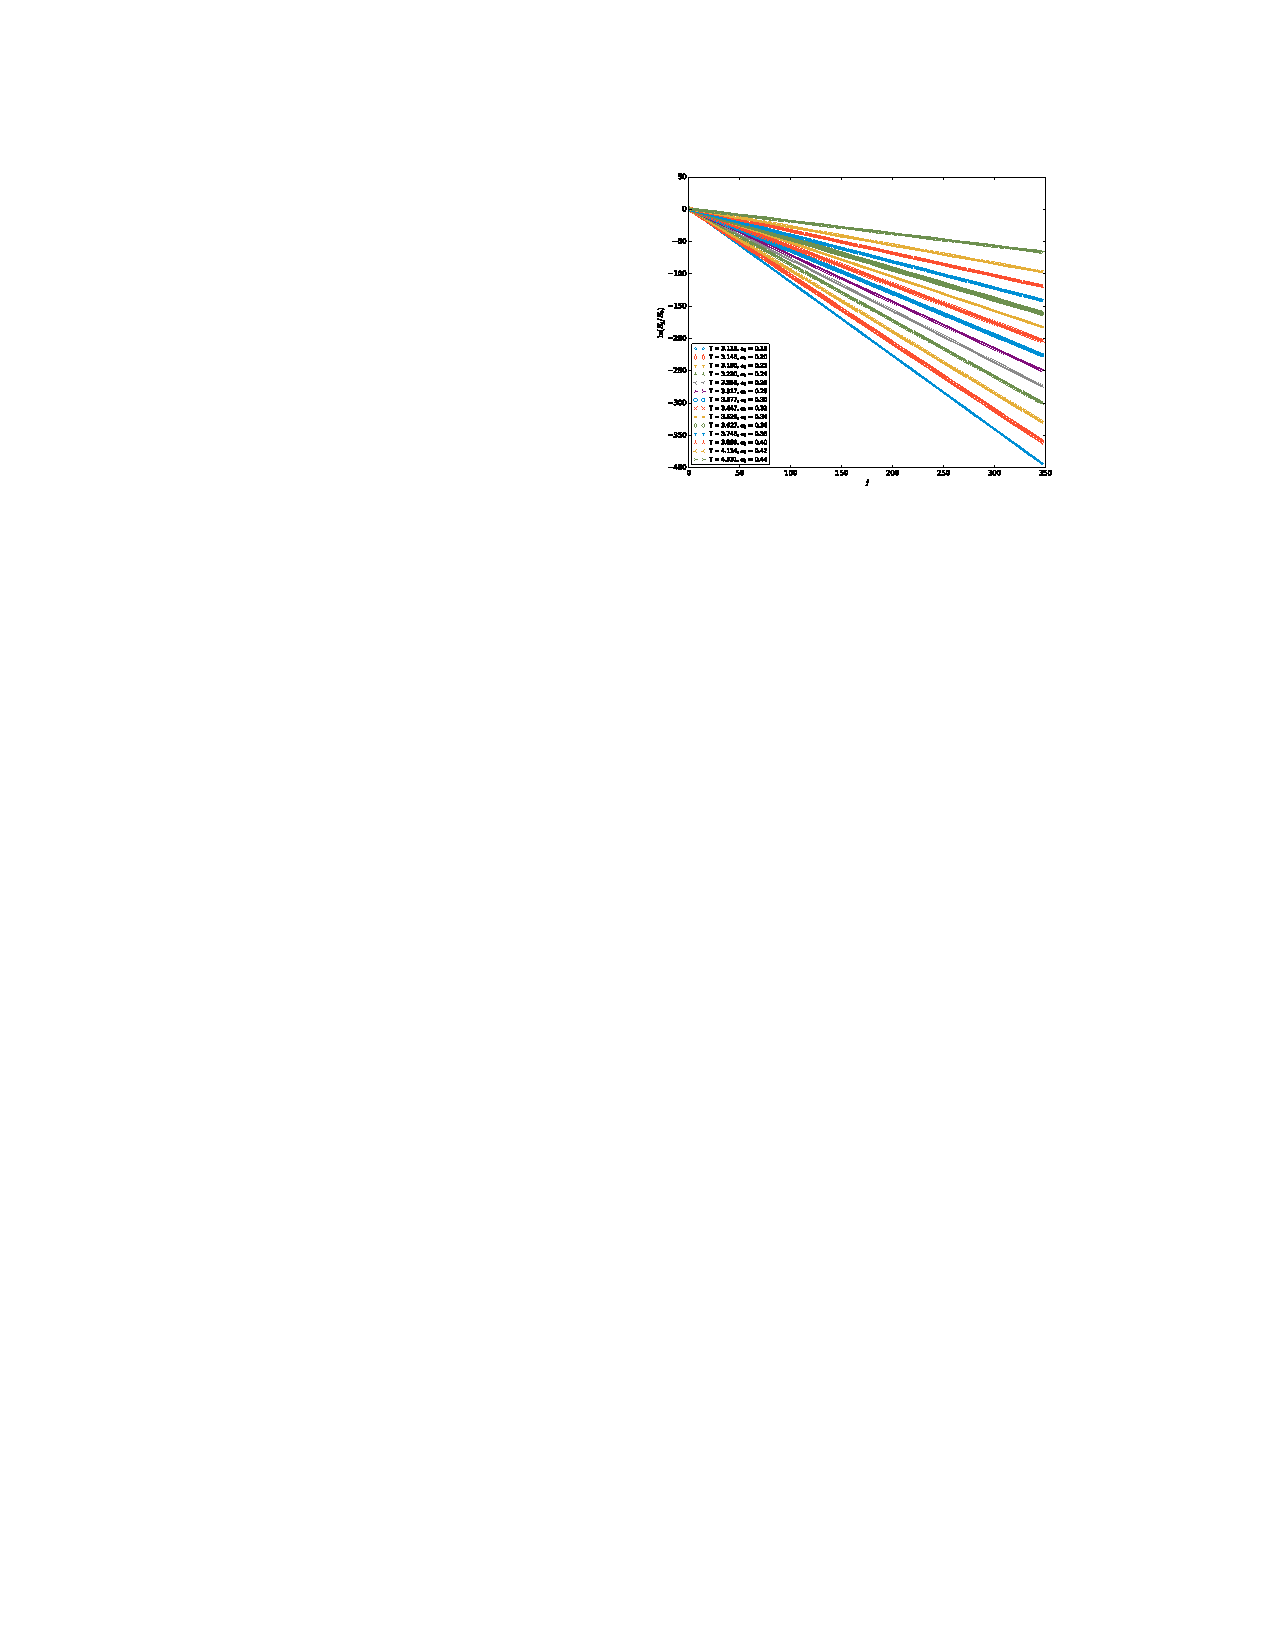
\includegraphics[width=\textwidth]{families}}
    \only<2>{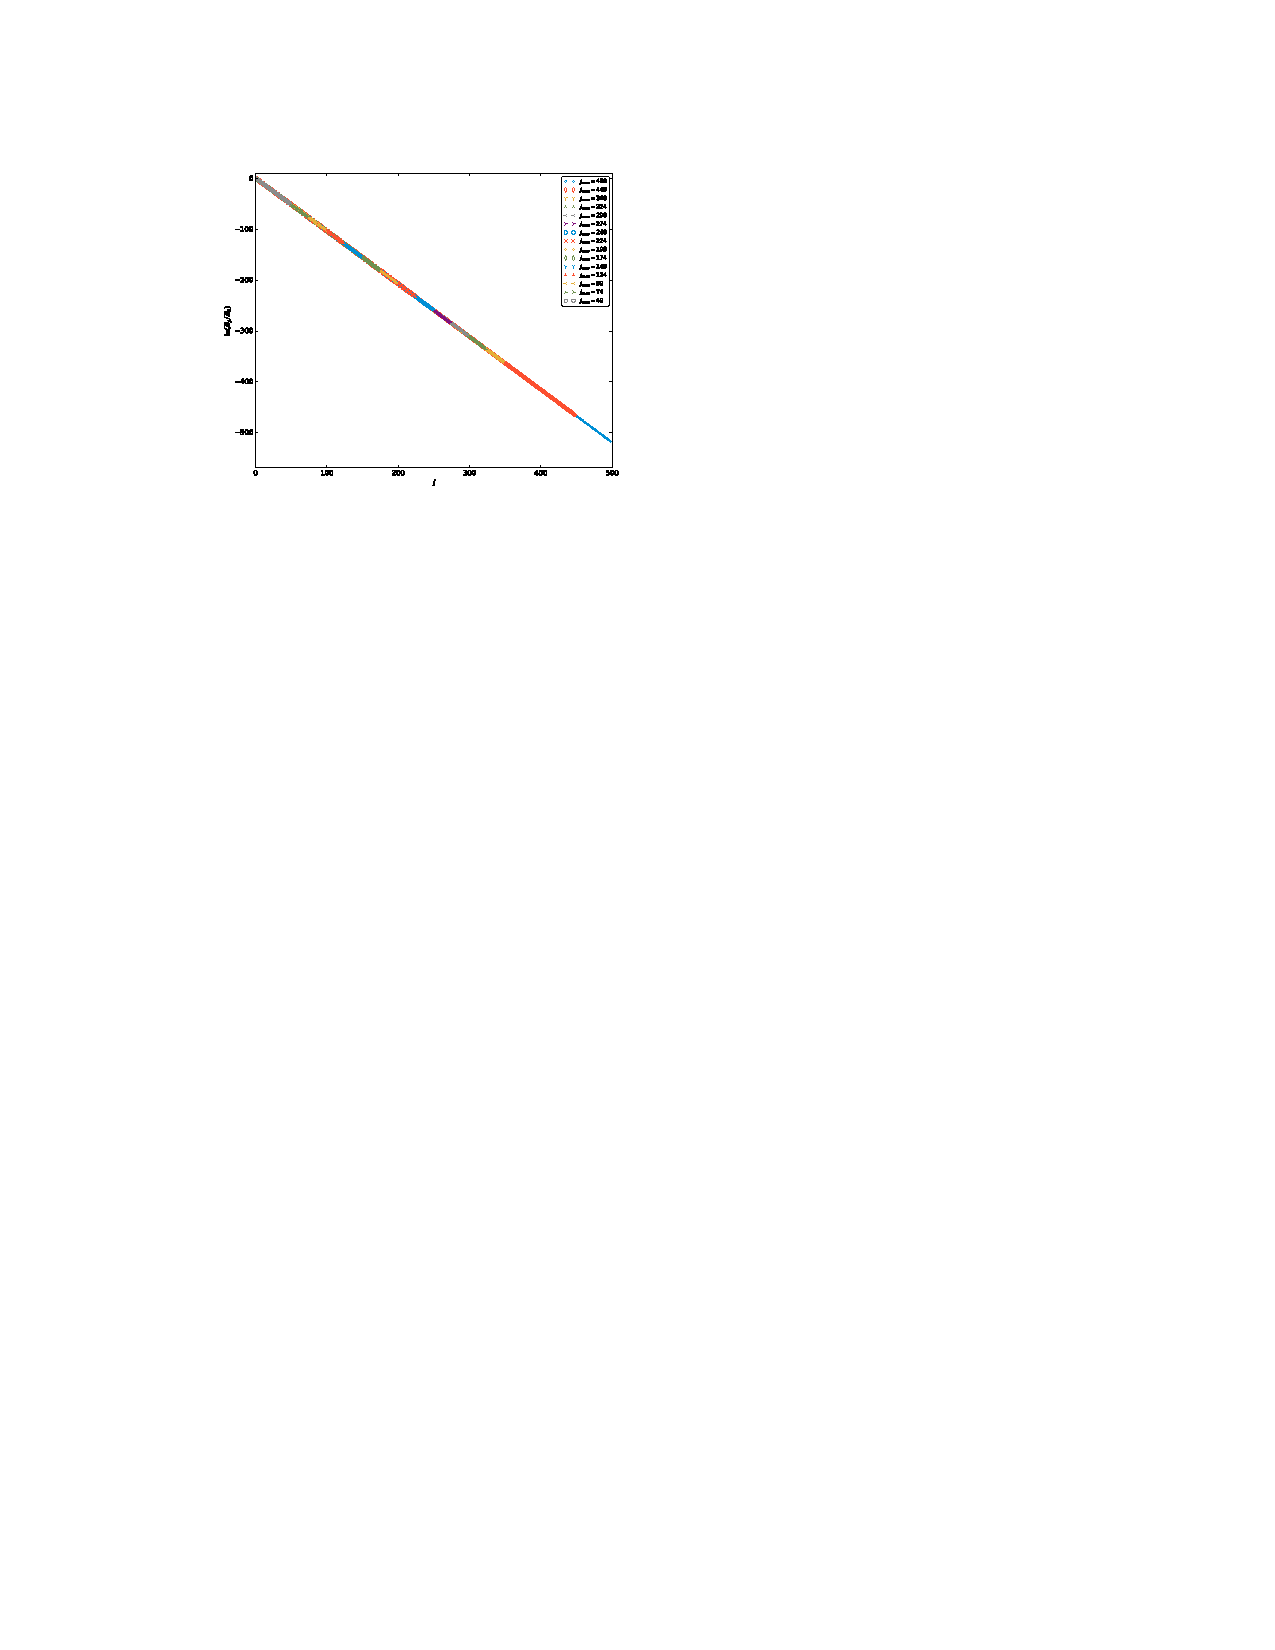
\includegraphics[width=\textwidth]{largejmax}}
  \end{figure}
  \end{columns}
 
}

%%%%%%%%%%%%%%%%%%%%%%%%%%%%%%%%%%%%%%%%%%%%%%

\subsection{High-Temperature Families}
\frame
{
  \frametitle{High-Temperature Families I}
  \bi
  \its Perturb by $\delta E$ $\to$ new solutions have energy $E + \delta E$, $N$, and $T + \delta T$
  \its Solve for updated values of $\alpha_j + \delta \alpha_j, \beta_j + \delta \beta_j$
  \its Use updated values as seeds to resolve QP equation
  \its Repeat process up to $T_{max}$\footnote<1->{{\scr Green {\it et al.}} [1507.08261]}
  \its<2->{{\bf Issue}: $\delta \alpha_j, \delta \beta_j$ become larger than $\alpha_j, \beta_j$ at high temperatures}
  \its<2->{No solutions that remain robust as $j_{max}$ increases}
  \ei
}

\frame
{
  \frametitle{High-Temperature Families II}
   \begin{figure}
    \centering
    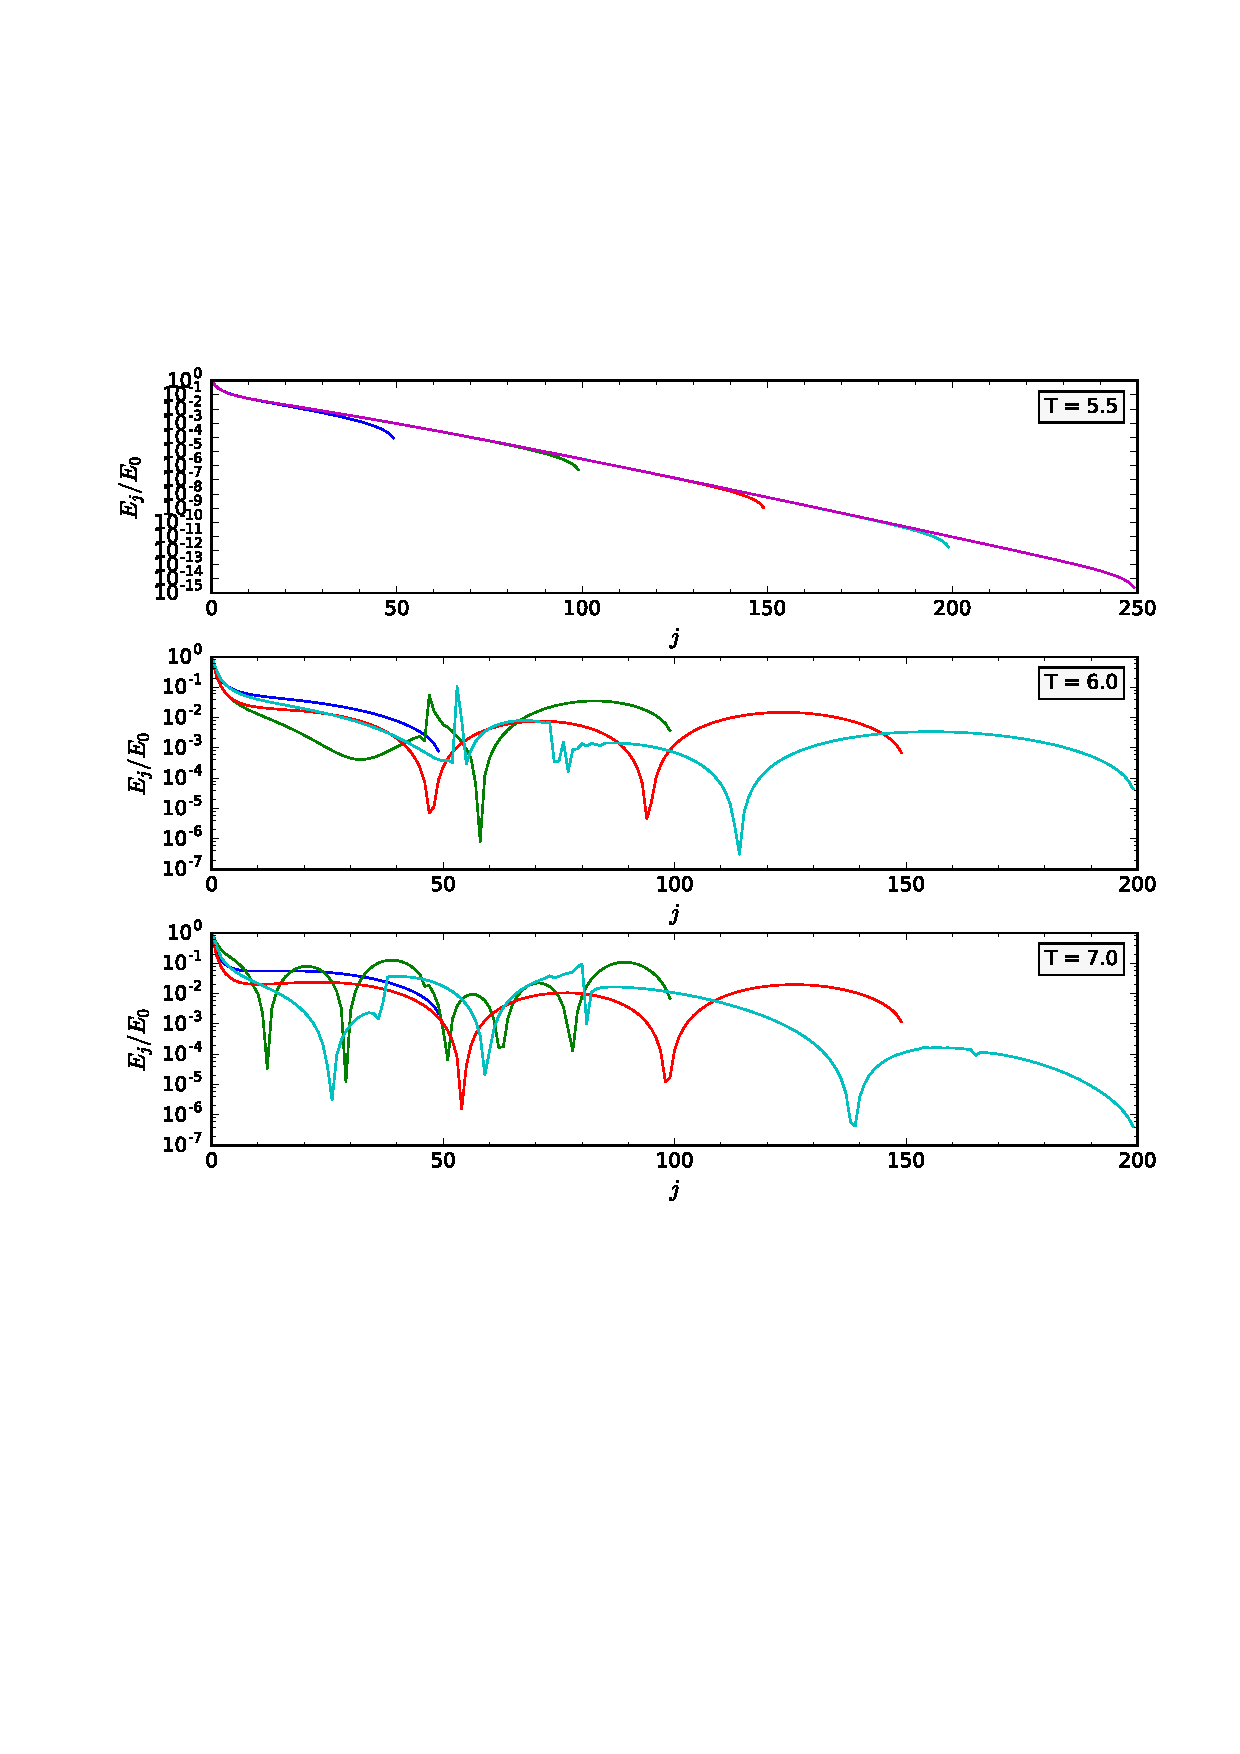
\includegraphics[scale=0.53]{constantTproj}
  \end{figure}
}

\frame
{
  \frametitle{High-Temperature Families III}
  \bi
  \its Alternative methods for finding high-T solutions explored 
  \its E.g. fit low $\jm$, high-T data to generate seeds for Newton-Raphson solver
     \ei
   \begin{overlayarea}{\textwidth}{0.65\textheight}
      \begin{figure}
      \centering
      \only<1-2>{
      \vspace{-0.13in}
      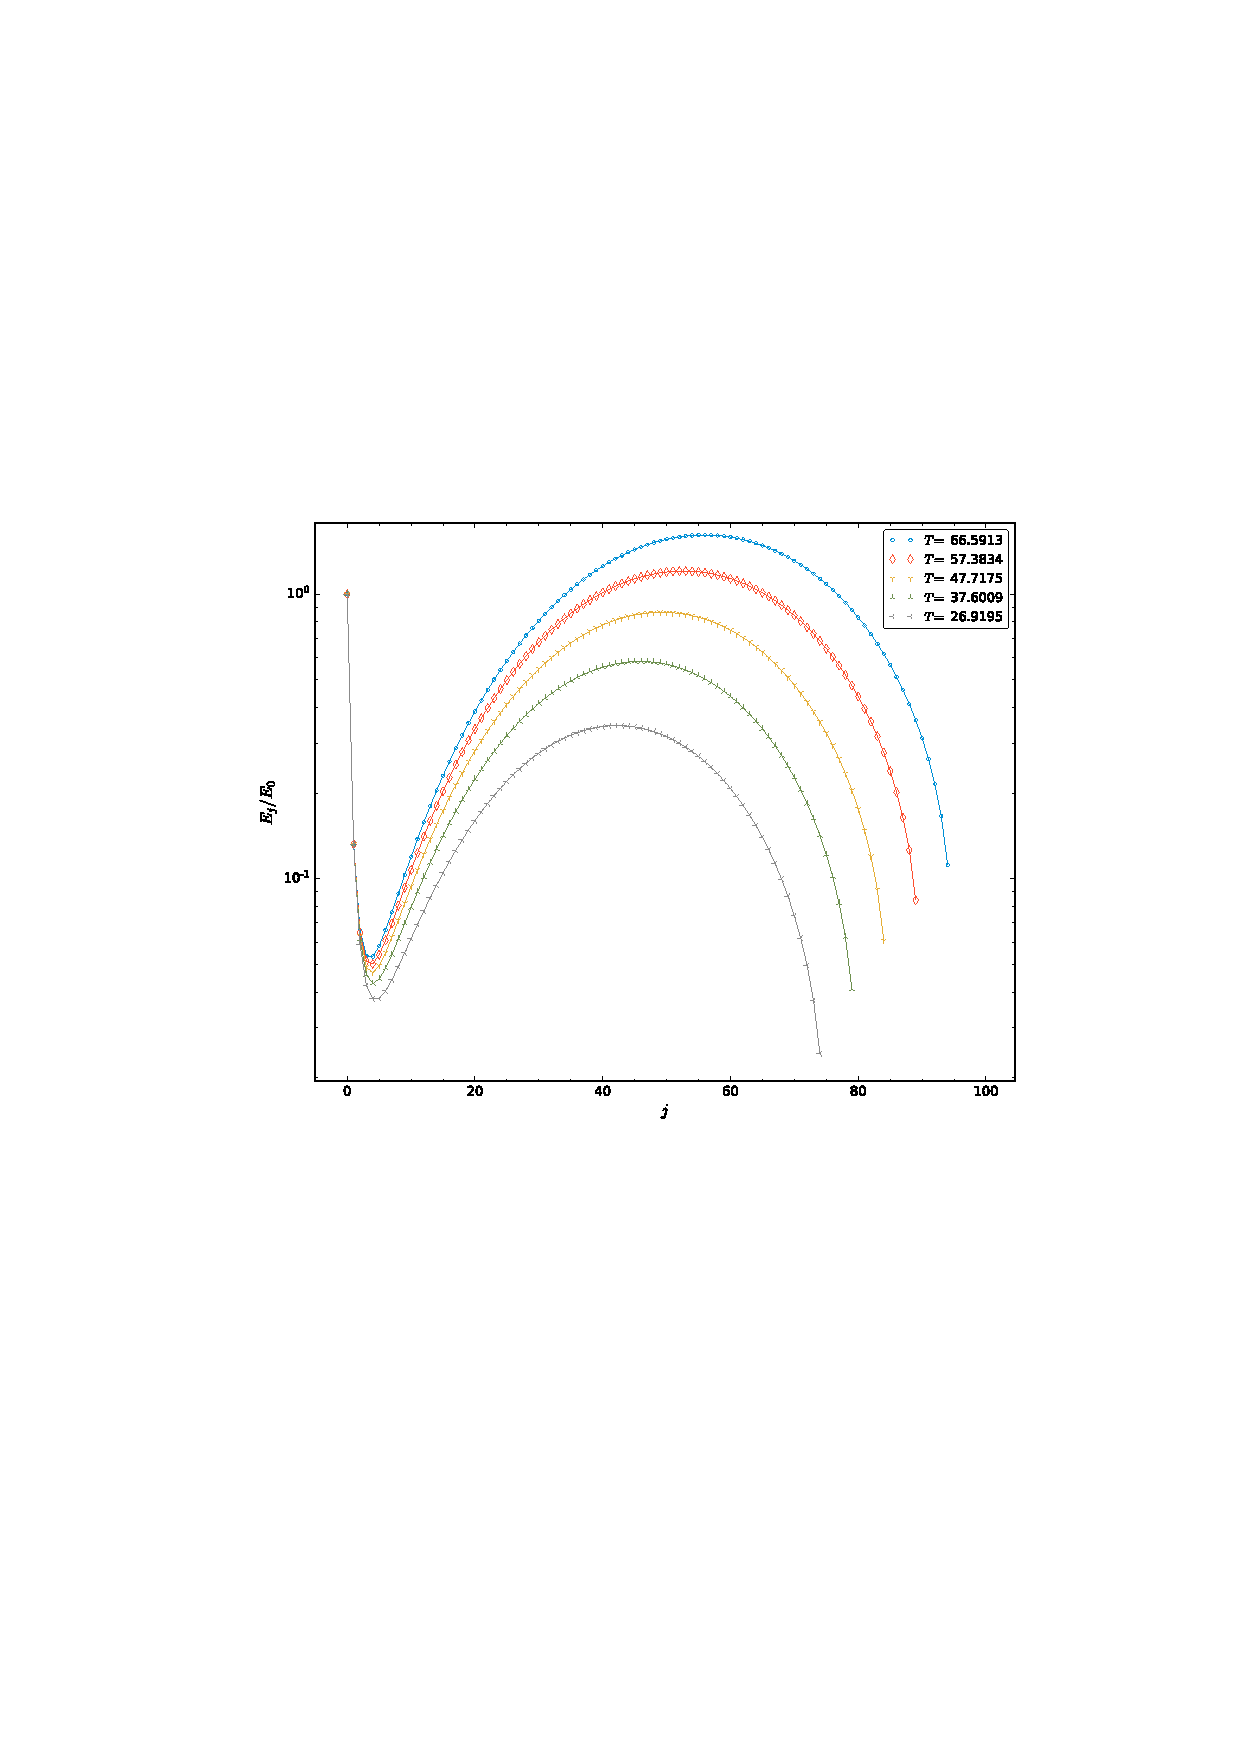
\includegraphics[scale=0.6]{highTseeds}
      }
      \end{figure}
  \end{overlayarea}
}

%%%%%%%%%%%%%%%%%%%%%%%%%%%%%%%%%%%%%%%%%%%%%%

\subsection*{}
\frame
{
  \frametitle{Results}
    \bi
    \its Low-T QP solutions robust as $\jm$ increases
    \its Not able to find evidence that high-T solutions continued to exist at large $\jm$ $\to$ possible reduction of space of QP
    \its {\bf Caveat}: focused on configurations where $\alpha_0 = 1$ $\to$ free to set dominant energy in any $\alpha_j$ $\to$ other configurations required for high temperatures?
    \its {\bf To do}: Motivation for temperature limit of $T \sim 5.5$?
    \its Perturbative system: massless scalar, static boundary conditions at $x = \pi/2$
    \its Extend to massive scalars, time-dependent boundary conditions $\to$ activation of non-normalizable modes
    \ei
}

%%%%%%%%%%%%%%%%%%%%%%%%%%%%%%%%%%%%%%%%%%%%%%
%%%%%%%%%%%%%%%%%%%%%%%%%%%%%%%%%%%%%%%%%%%%%%

\section{Driven Scalars in AdS}
\frame[c, noframenumbering, fragile=singleslide]
{
  \frametitle{}
  \begin{center}
    \begin{mybox}[]
    B Cownden, {\it Examining Instabilities Due to Driven Scalars in AdS}, \verb|JHEP_252P_0420| , [1912.07143].
    \end{mybox}
  \end{center}
}

%%%%%%%%%%%%%%%%%%%%%%%%%%%%%%%%%%%%%%%%%%%%%%

\subsection{Extending TTF to Driven Scalars}
\frame
{
  \frametitle{Extending TTF to Driven Scalars}
  \bi
  \its Driven scalars $\to$ equation for $\phi_1$ has inhomogeneous term at $x = \pi / 2$
  \its<2->{Examine scaling behaviour as $x \to \pi/2$: $\Phi^+(x) \sim (\cos x)^{\Delta^+}$ and $\Phi^-(x) \sim (\cos x)^{\Delta^-}$}
  \its<3->{Scalar field is linear combination of both kinds of modes}
  \its<3->{\alert<3>{$e_j(x)$} are same eigenfunctions of AdS \& have eigenvalues \alert<3>{$\omega_j = (2j + \Delta^+)$}}
  \its<4->{\alert{$E_\alpha(x)$} are hypergeometric functions with frequencies \alert{$\omega_\alpha$} from $\mc F(t)$}
  \ei
  \vspace{-0.2in}
  \begin{overlayarea}{\textwidth}{0.25\textheight}
  \begin{align*}
  \only<1>{
  	\p^2_t \phi_1 + \hat L \phi_1 = \delta(x - \pi/2) \mc F(t)
  }
  \only<2>{
    \Phi^+(x) \equiv \text{``normalizable''} \quad & \quad \Phi^-(x) \equiv \text{``non-normalizable''}
    }
  \only<3->{
    \phi_1(t,x) = \sum_{j=0}^\infty a_j(t) \cos & \left(\alert<3>{\omega_j} t + b_j (t)\right) \alert<3>{e_j(x)} + \sum_{\alpha = 0}^\infty \mathcal A_\alpha(t) \cos \left( \alert<4>{\omega_\alpha} t + \mathcal B_\alpha \right) \alert<4>{E_\alpha (x)} \\
    & \alert<3>{\Delta^\pm = \frac{d}{2} \pm \frac{1}{2} \sqrt{d^2 + 4m^2}}
    }
  \end{align*}
  \end{overlayarea}
  \vspace{0.3in}
}

%%%%%%%%%%%%%%%%%%%%%%%%%%%%%%%%%%%%%%%%%%%%%%

\subsection{Resonant Contributions}
\frame
{
  \frametitle{Resonant Contributions I}
  \bi
  \its $\mc O(\epsilon^3)$: source terms for resonant contributions $\to$ examine resonance conditions 
  \its<2->{{\bf Unforced}: restrictions on indices and mass value \uncover<3->{$\to$ \alert<3>{two channels vanish numerically}}}
  \its<4->{One \alert{non-vanishing} channel}
  \ei
  
  \begin{overlayarea}{\textwidth}{0.5\textheight}
  \only<1-4>{
  \vspace{0.2in}
  \begin{align*}
 \alert<3>{\omega_i + \omega_j + \omega_k} &\alert<3>{= \omega_\ell} \uncover<2->{\alert<3>{\quad \Rightarrow \quad i + j + k = \ell - \Delta^+  \in \mathbb{Z}^+}} \\
  \alert<3>{\omega_i - \omega_j - \omega_k} &\alert<3>{= \omega_\ell} \uncover<2->{\alert<3>{\quad \Rightarrow \quad i - j - k = \ell + \Delta^+  \in \mathbb{Z}^+}} \\
  \alert<4>{\omega_i + \omega_j - \omega_k} &\alert<4>{= \omega_\ell} \uncover<2->{\alert<4>{\quad \Rightarrow \quad i + j = k + \ell \, \in \mathbb{Z}^+}}
  \end{align*}
  }  
  \end{overlayarea}
}

\frame
{
   \frametitle{Resonant Contributions II} 
   \bi
   \its Sum over $i$, $j$ with $i + j \leq \ell$ (dots: $a_\ell^3$, triangles: $a_i^2 a_\ell$, X: $a_i a_j a_{i + j -\ell}$)
   \ei
   \begin{figure}
   \centering
    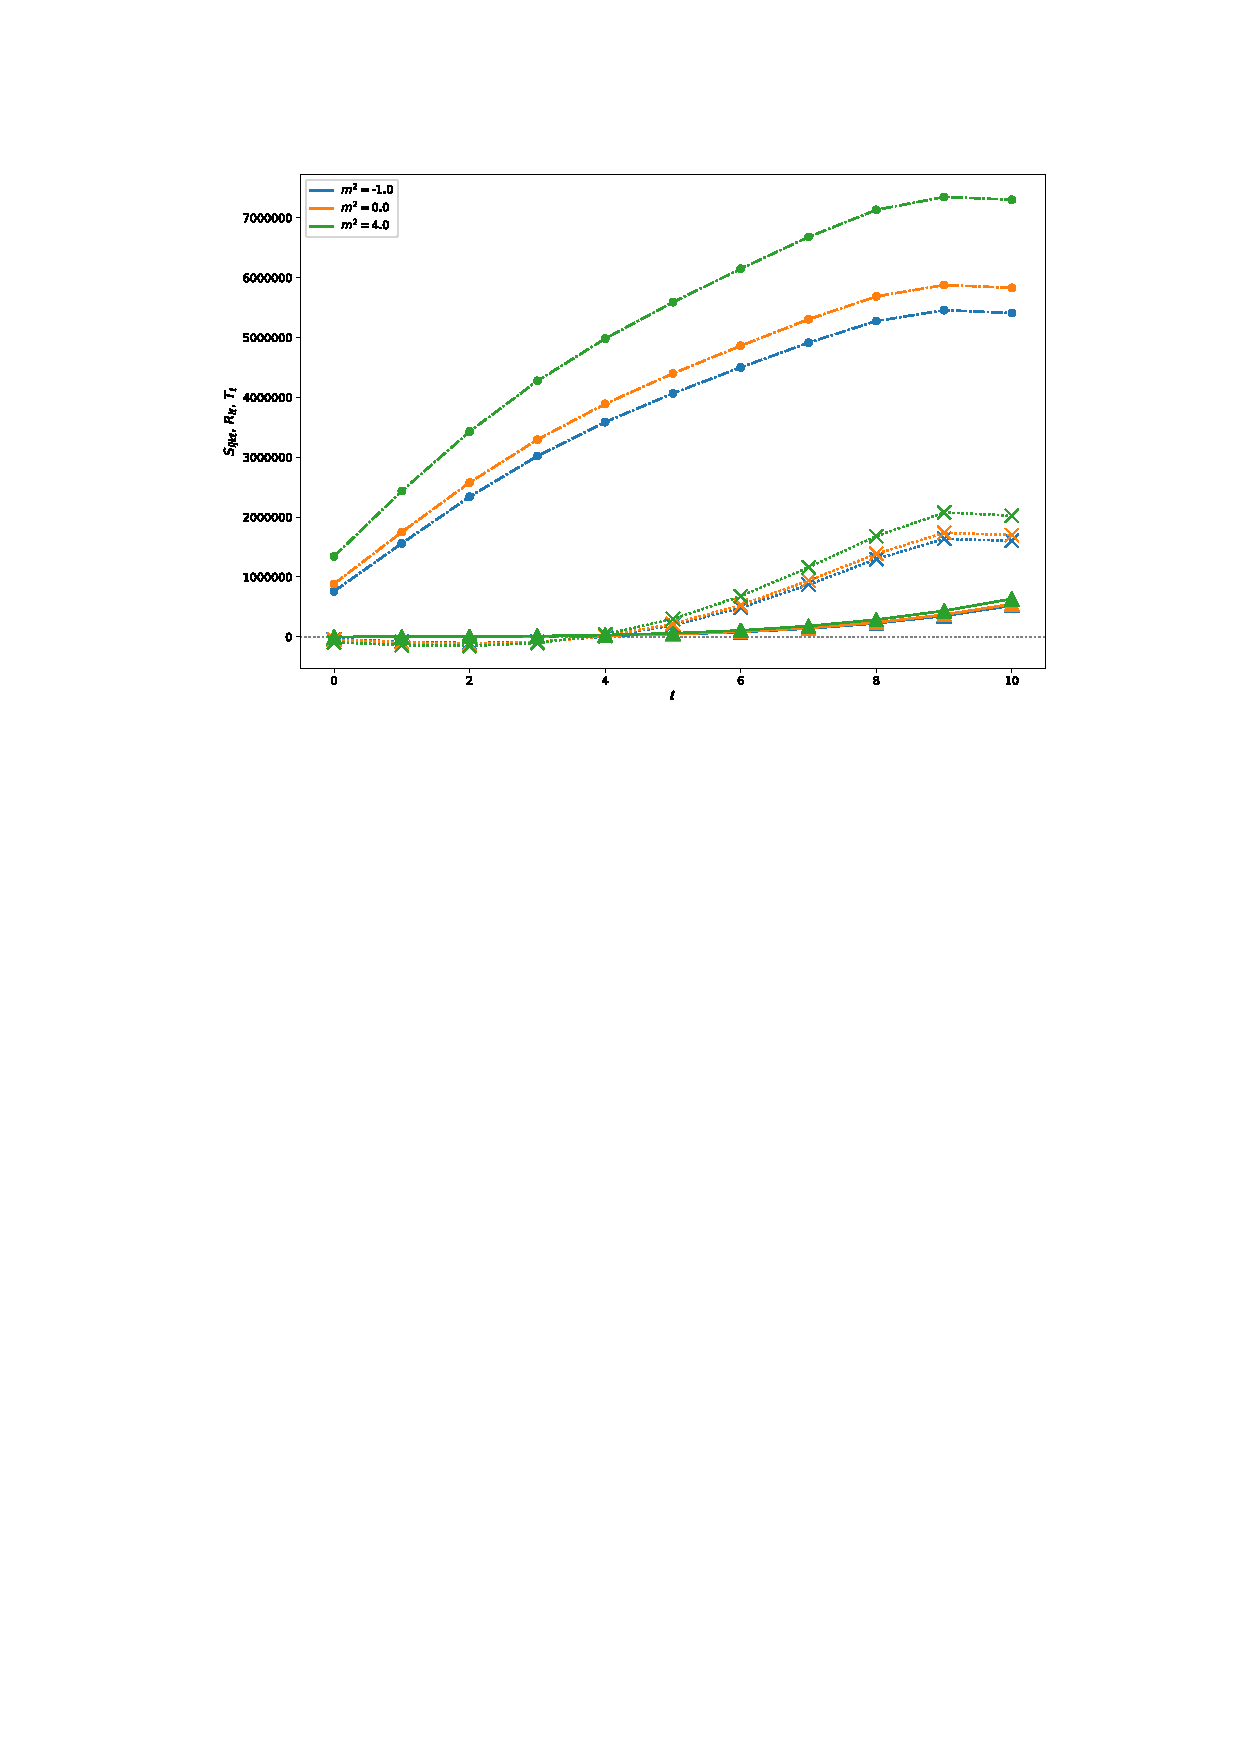
\includegraphics[scale=0.75]{norm} 
    \end{figure}
}
   

%%%%%%%%%%%%%%%%%%%%%%%%%%%%%%%%%%%%%%%%%%%%%%

\subsection{Special Values of Non-normalizable Frequencies}
\frame
{
  \frametitle{Special Values of Non-normalizable Frequencies}
  \begin{columns}
  \column{0.4\textwidth}
  \bi
  \its {\bf Forced}: $\omega_\alpha$ set by driving term
  \its\alert<1>{Single frequency}: $\omega_\alpha = \bar\omega$ $\to$ one channel
  \its<2->{\alert<2>{Add to integer}: $\bar\omega_1 + \bar\omega_2 = 2n$ $\to$ three channels}
  \ei

  \uncover<1->{
  \begin{overlayarea}{\textwidth}{0.25\textheight}
  \[
  	\only<1>{\alert{\omega_i + \bar\omega - \bar\omega = \omega_\ell}} 
  	\only<2>{
	\begin{array}{ll}
	 	 \alert<2>{(++): \omega_i + 2n = \omega_\ell \quad \forall \, \ell \geq n} & \\
	 	 \alert<2>{(+-):  \omega_i - 2n = \omega_\ell \quad \forall \, n} & \\
		 \alert<2>{(-+): - \omega_i + 2n = \omega_\ell \quad \forall \, n \geq \ell + d} & 
	\end{array}
	}
  \]
  \end{overlayarea}
 }
 
 \only<1>{\vspace{0.1in}}
  \column{0.6\textwidth}
  	\begin{figure}
	\centering
	\only<1>{
	\vspace{-0.2in}
	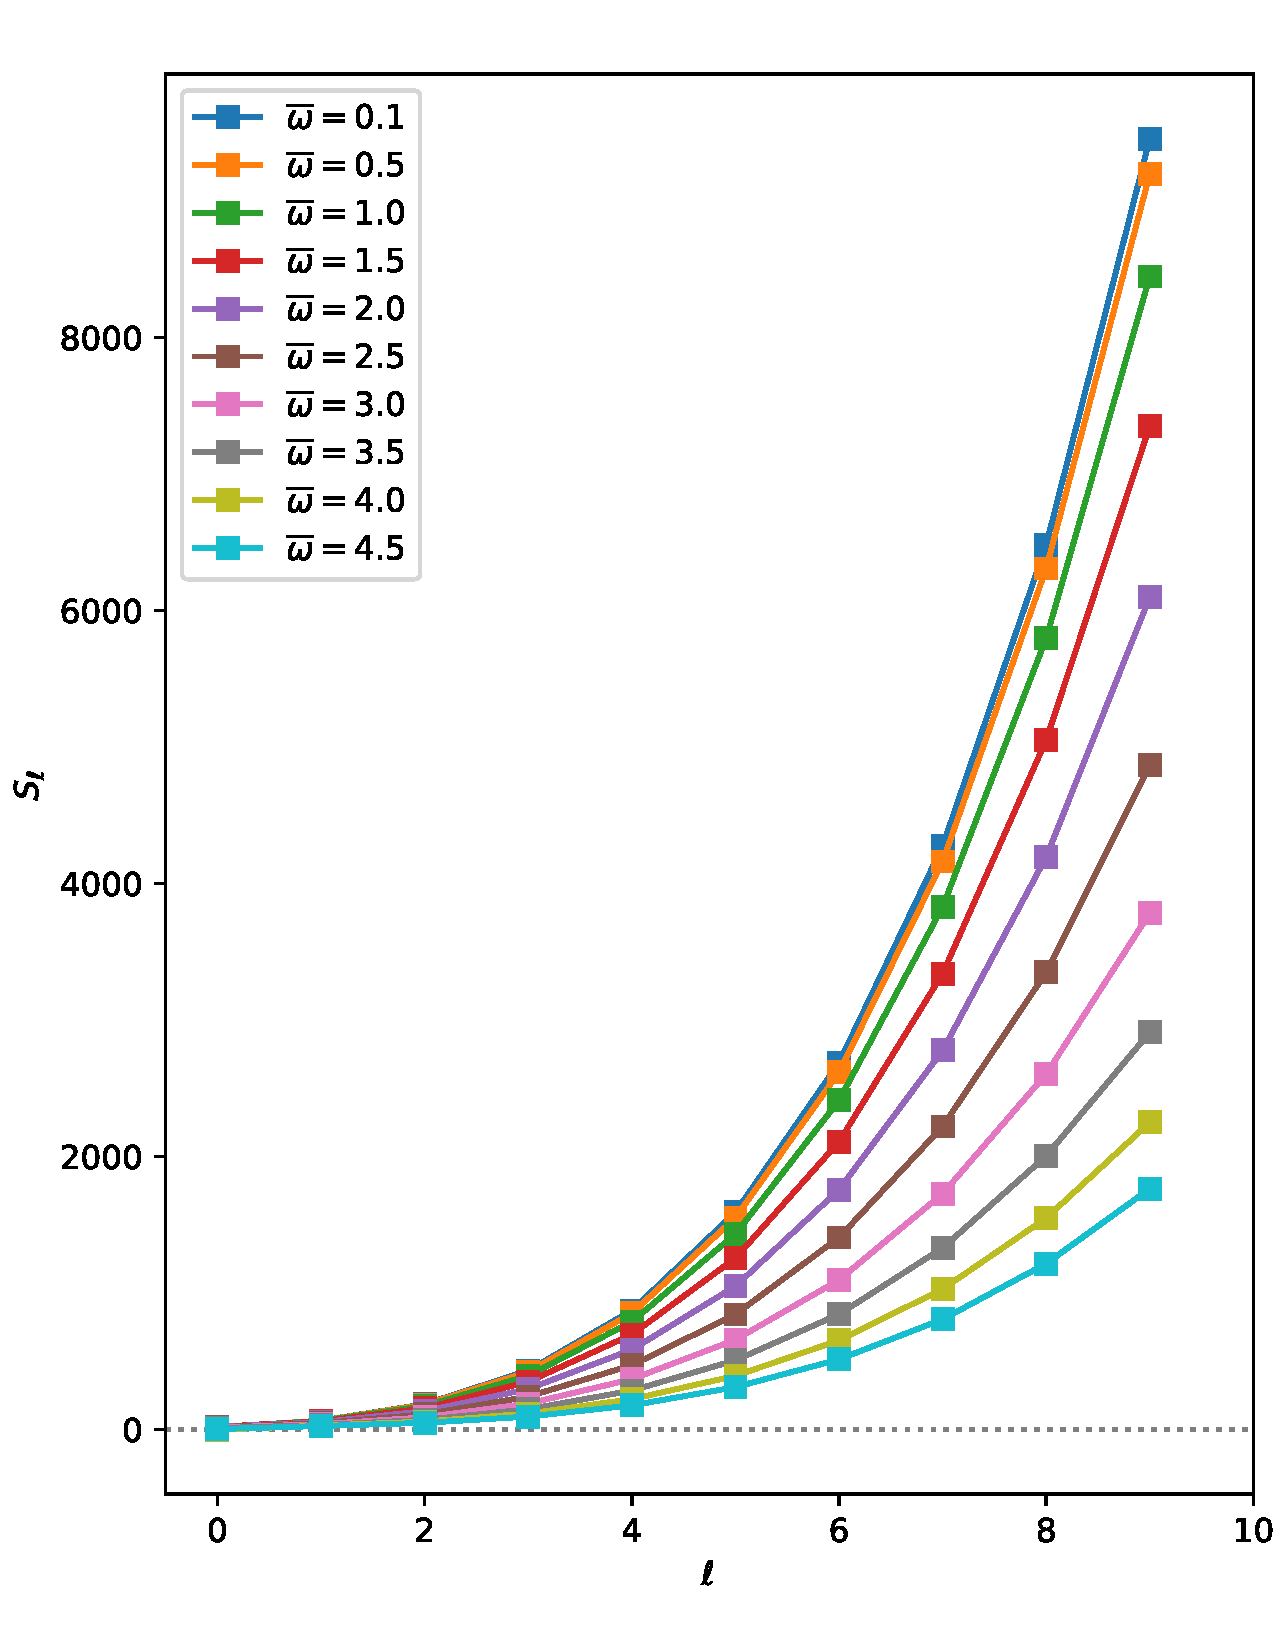
\includegraphics[width=0.87\textwidth]{equalNNm0}
	}
	\only<2>{
	\vspace{-0.1in}
	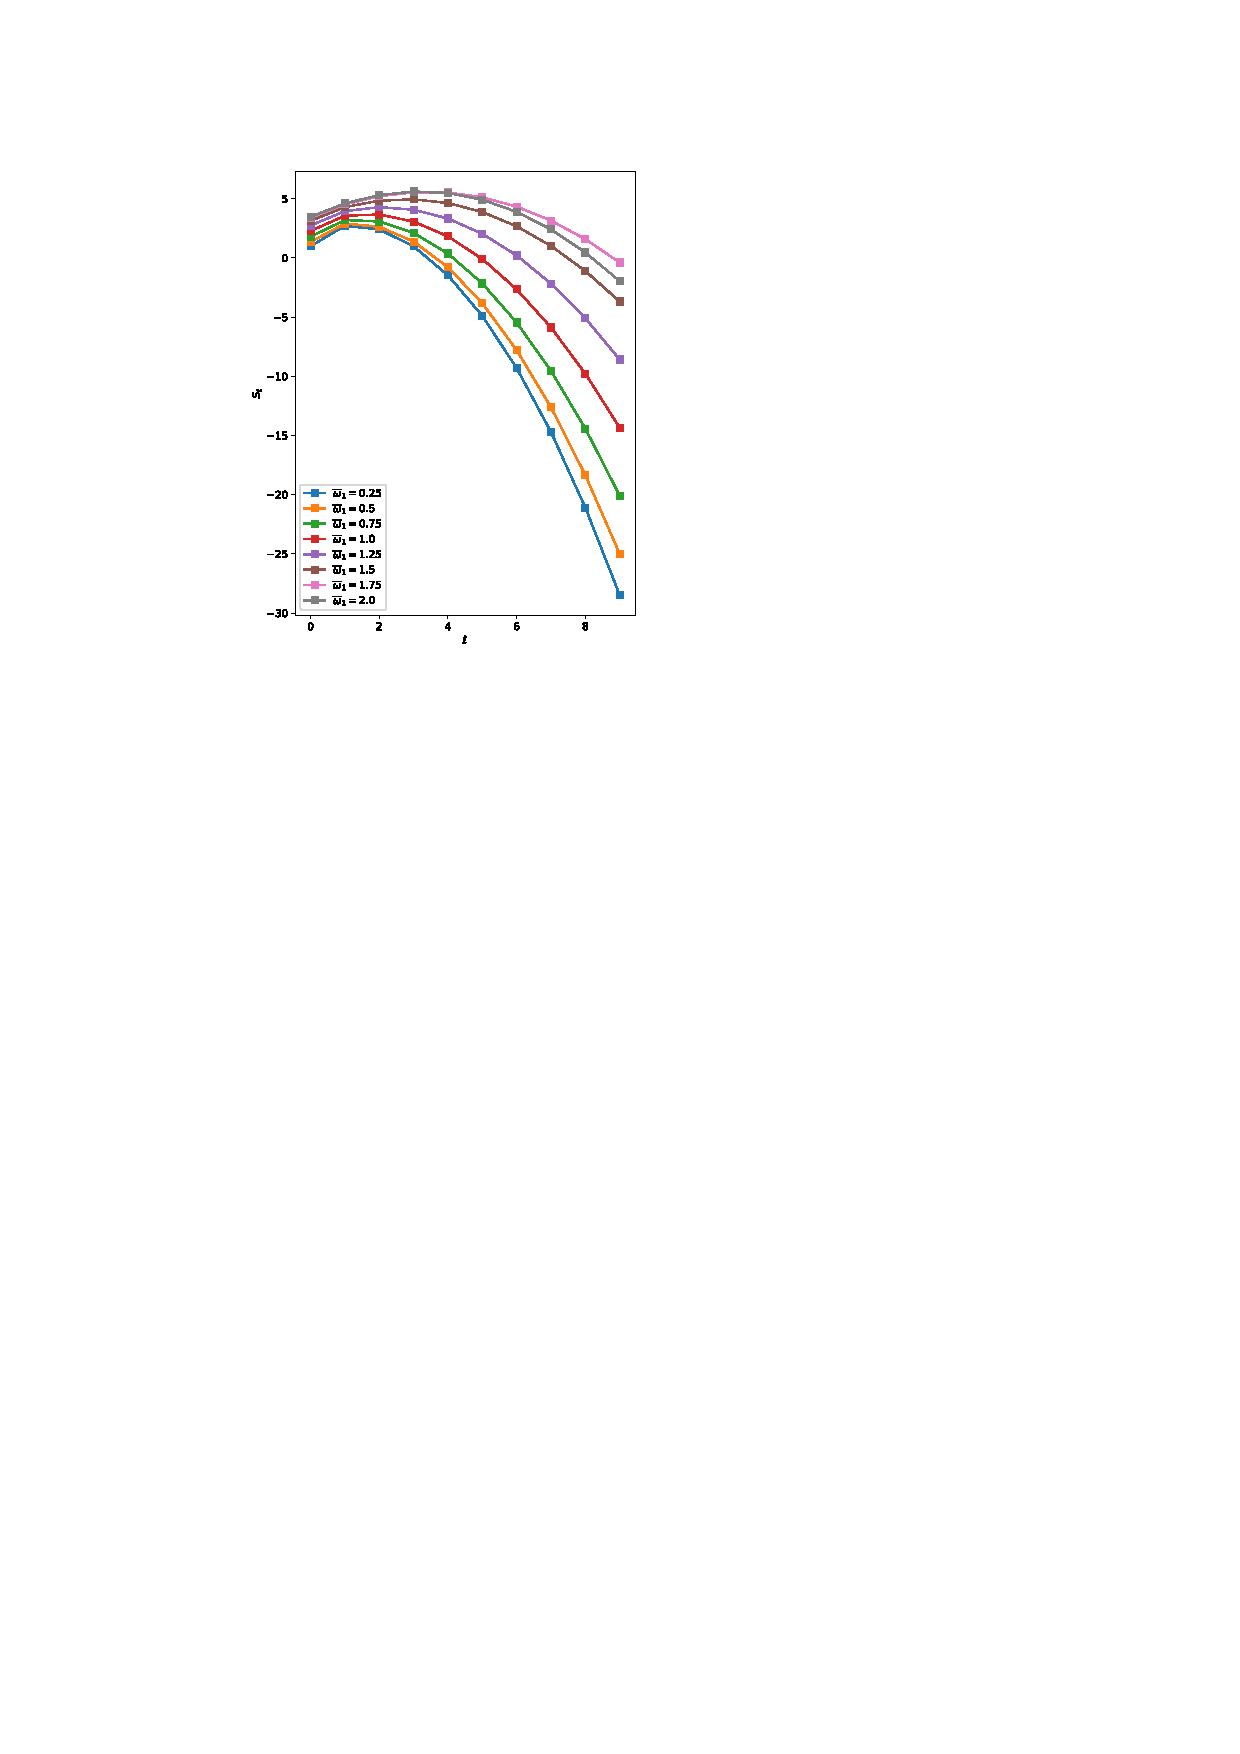
\includegraphics[width=0.85\textwidth]{NNsum4m0}
	}
	\end{figure}
  \end{columns}
 }

\frame
{
  \frametitle{Flow Equations}
  \bi
  \its Source terms give flow equations for amplitude/phase of normalizable modes
  \its No naturally vanishing resonances, {\it c.f.} static boundary conditions
  \its E.g. single frequency $\to$ \alert<1>{single channel} $\to$ equations decouple
  \its<2->{E.g. add to integer $\to$ sum all \alert{three channels} $\to$ equations are coupled with single power of normalizable amplitude}
  \ei
  \vspace{-0.2in}
  \begin{overlayarea}{\textwidth}{0.5\textheight}
  	\begin{align*}
	\only<1>{
	\frac{2 \omega_\ell}{\epsilon^2} \frac{d a_\ell}{dt} = 0 \qquad \text{and} \qquad \frac{2 \omega_\ell}{\epsilon^2} \frac{db_\ell}{dt} = \alert{f^{(\ell)}} \mathcal A^2_{\bar \omega} 
	}
	\only<2>{
	&\frac{2 \omega_\ell}{\mathcal A_1 \mathcal A_2 \epsilon^2} \frac{d a_\ell}{dt} = \sum_{(++)} \alert{f^{(\ell)}_{(++)}} a_{n - \ell - d} \sin \left(b_{n-\ell - d} - \mathcal B_1 - \mathcal B_2\right) \\
	& \!\!\!\! + \sum_{(+-)} \alert{f^{(\ell)}_{(+-)}} a_{\ell - n} \sin \left( b_{\ell - n} - \mathcal B_1 - \mathcal B_2 \right) + \sum_{(-+)} \alert{f^{(\ell)}_{(-+)}} a_{\ell + n} \sin \left( b_{\ell + n} - \mathcal B_1 - \mathcal B_2 \right) \\
	 & \frac{2 \omega_\ell a_\ell}{\mathcal A_1 \mathcal A_2 \epsilon^2} \frac{db_\ell}{dt} = \alert{f^{(\ell)}} a_\ell + \sum_{(++)} \alert{f^{(\ell)}_{(++)}} a_{n - \ell - d} \cos \left(b_{n-\ell - d} - \mathcal B_1 - \mathcal B_2\right) \\
	 & \!\!\!\! + \sum_{(+-)} \alert{f^{(\ell)}_{(+-)}} a_{\ell - n} \cos \left(b_{\ell - n} - \mathcal B_1 - \mathcal B_2 \right) + \sum_{(-+)} \alert{f^{(\ell)}_{(-+)}} a_{\ell + n} \cos \left( b_{\ell + n} - \mathcal B_1 - \mathcal B_2 \right)
	}
	\end{align*}
  \end{overlayarea}
    \vfill
}

%%%%%%%%%%%%%%%%%%%%%%%%%%%%%%%%%%%%%%%%%%%%%%

\subsection*{}
\frame
{
  \frametitle{Results}
  \bi
  \its Confirm two of three resonant channels vanish for massive scalar (all normalizable)\footnote{{\scr Biasi {\it et al.} [1810.04753]}}
  \its First TTF formulation with time-dependent boundary conditions
  \its No naturally-vanishing source terms $\to$ sum resonant channels
  \its Some flow equations decouple amplitude/phase variables $a_\ell(t)$, $b_\ell(t)$
  \its {\bf Note}: normalizable modes are still present $\to$ sum all contributions
  \its {\bf Further work}: quasi-periodic solutions\footnote{{\scr Carracedo {\it et al.} [1612.07701]}}? Conserved quantities? Energy cascades?
  \ei

}

%%%%%%%%%%%%%%%%%%%%%%%%%%%%%%%%%%%%%%%%%%%%%%
%%%%%%%%%%%%%%%%%%%%%%%%%%%%%%%%%%%%%%%%%%%%%%

{
  \AtBeginSection[]{}
\section{Conclusions}
\frame
{
   \frametitle{Conclusions}
   \bi
   \its Examine the stability of AdS to scalar field collapse in various dimensions in perturbative \& non-perturbative regimes $\to$ addition of time-dependent boundary conditions
   \its<2->{Constructed phase diagram of scalar field collapse in AdS$_5$ $\to$ two new phases on ``shorelines'' $\to$ non-perturbative regime only}
   \its<2->{First evidence of weakly chaotic evolution of scalars in AdS$_5$}
   \its<3->{Verified low-T QP solutions are robust in the $j_{max} \to \infty$ limit}
   \its<3->{No evidence of high-T QP solutions for $\alpha_0 = 1$ family}
   \its<4->{Developed perturbative theory for massive scalars with time-dependent boundary conditions}
   \its<4->{Derived flow equations for amplitude/phase variables for some choices of driving term $\to$ evaluated source terms numerically}
   \ei
}
\section*{}
\frame[noframenumbering]
{
   \frametitle{Thanks}
   \begin{itemize}
   \its Supervisor: Andrew Frey
   \its PhD Committee: Derek Krepski, Gabor Kunstatter, Robert Mann, Khodr Shamseddine
   \its Co-authors: Nils Deppe
   \its University of Winnipeg and University of Manitoba
   \its Westgrid \& Compute Canada
   \end{itemize}
}

\frame[noframenumbering]
{
  \frametitle{References}
  \bi
  \its J. Maldacena, \emph{The Large N limit of superconformal field theories and supergravity}, Int. J. Theor. Phys. 38 (1999) 1113-1133, [hep-th/9711200].
  \its P. Bizo\'n and A. Rostworowski, \emph{On weakly turbulent instability of anti-de Sitter space}, Phys. Rev. Lett. 107 (2011) 031102, [1104.3702]. 
  \its M. Choptuik, \emph{Universality and scaling in gravitational collapse of a massless scalar field}, Phys. Rev. Lett. 70 (1993) 9-12. 
  \its N. Deppe and A. R. Frey, \emph{Classes of Stable Initial Data for Massless and Massive Scalars in Anti-de Sitter Spacetime}, JHEP 12 (2015) 004, [1508.02709]. 
  \its R. Brito, V. Cardoso, and J. V. Rocha, \emph{Interacting shells in AdS spacetime and chaos}, Phys. Rev. D94 (2016), no. 2 024003, [1602.03535]. 
  \its N. Deppe, A. Kolly, A. R. Frey, and G. Kunstatter, \emph{Black Hole Formation in AdS Einstein-Gauss-Bonnet Gravity}, J. High Energ. Phys. (2016) 2016: 87, [1608.05402].
  \its A. Buchel, S. L. Liebling, and L. Lehner, \emph{Boson Stars in AdS Spacetime}, Phys. Rev. D87 (2013) 123006, [1304.4166].
 \ei
}

\frame[noframenumbering]
{
  \frametitle{References}
  \bi
  \its V. Balasubramanian, A. Buchel, S. R. Green, L. Lehner, and S. L. Liebling, \emph{Holographic Thermalization, Stability of Anti-de Sitter Space, and the Fermi-Pasta-Ulam Paradox}, Phys. Rev. Lett. 113 (2014) 071601, [1403.6471].
  \its B. Craps, O. Evnin, and J. Vanhoof, \emph{Renormalization group, secular term resummation and AdS (in)stability}, JHEP 10 (2014) 048, [1407.6273].
  \its B. Craps, O. Evnin, and J. Vanhhof, \emph{Renormalization, averaging, conservation laws and AdS (in)stability}, J. High Energ. Phys. 1501 (2015) 108, [1412.3249].
  \its S. R. Green, A. Maillard, L. Lehner, and S. L. Liebling, \emph{Islands of stability and recurrence times in AdS}, Phys. Rev. D92 (2015) 084001, [1507.08261].
    \its A. Biasi, B. Craps, and O. Evnin, \emph{Energy Returns in Global AdS$_4$}, [1810.04753].
  \its P. Carracedo, J. Mas, D. Musso and A. Serantes, \emph{Adiabatic pumping solutions in global AdS}, JHEP 05 (2017) 141, [1612.07701].
  \ei
}
}

\end{document}

%%%%%%%%%%%%%%%%%%%%%%%%%%%%%%%%%%%%%%%%%%%%%%
%%%%%%%%%%%%%%%%%%%%%%%%%%%%%%%%%%%%%%%%%%%%%%

